\documentclass[output=paper,colorlinks,citecolor=brown]{langscibook}
\ChapterDOI{10.5281/zenodo.18845932}
\author{Jorge R. Valdés Kroff\orcid{0000-0002-3943-5496}\affiliation{University of Florida} and Hannah G. Treadway\orcid{0000-0001-6244-7674}\affiliation{University of Florida} and Rosa E. Guzzardo Tamargo\orcid{0000-0002-3074-8680}\affiliation{University of Puerto Rico at Río Piedras} and Paola E. Dussias\orcid{0000-0002-9481-7489}\affiliation{Pennsylvania State University}}
\title{Sensitivity to codeswitching asymmetries in second language processing}

\abstract{Some Spanish-English bilingual communities in the US and Puerto Rico show a preference for codeswitched verb compounds involving the progressive auxiliary, \textit{estar}. These switches are produced before or after the auxiliary with similar levels of frequency and acceptability. In contrast, verb phrases involving the perfect auxiliary, \textit{haber}, show a clear dispreference for switches that occur within the verb compound. This same asymmetry is found in real-time sentence processing in early Spanish-English bilinguals and late second language (L2) speakers of English. We test 61 late L2 speakers of Spanish immersed in a region where Spanish-English bilingual speech is present to determine whether they exhibit online sensitivity to this asymmetry during online reading. Results indicate that L2 Spanish speakers demonstrate a sustained asymmetric pattern of sensitivity in later stages of reading, but only if they engaged in a session where they answered comprehension questions. Another L2 Spanish group that completed forced-choice grammaticality judgments while reading the same sentence constructions did not show sensitivity to the same asymmetry. We interpret our findings to point towards an important role for experience with exposure to community-based code-switching patterns to successfully acquire and deploy during online sentence processing.
\keywords{codeswitching, eye-tracking, bilingual verb phrase}
}

\lehead{J. R. Valdés Kroff, H. G. Treadway, R. E Guzzardo Tamargo and P. E. Dussias}

%move the following commands to the "local..." files of the master project when integrating this chapter
% \usepackage{tabularx}
% \usepackage{langsci-optional}
% \usepackage{langsci-gb4e}
% \usepackage{multirow}
% \usepackage[hyphens]{url}
% \bibliography{localbibliography}
% \newcommand{\orcid}[1]{}

\IfFileExists{../localcommands.tex}{
   \addbibresource{../localbibliography.bib}
   \usepackage{tabularx,multicol}
\usepackage{url}
\urlstyle{same}

 
\usepackage{langsci-optional}
\usepackage{langsci-lgr}
\usepackage{langsci-gb4e}

\usepackage{multirow}
\usepackage{cleveref}
\usepackage{subfigure}
\usepackage{langsci-branding}

   \input{../localcommands}
   \input{../localhyphenation}
   \boolfalse{bookcompile}
   \togglepaper[5]%%chapternumber
}{}

\begin{document}
\maketitle


\section{Introduction}
Bilinguals in the presence of other bilinguals may engage in codeswitching, the fluid use of both languages within bilingual speech or text. Bilinguals rarely code-switch accidentally when in the presence of monolinguals or in pragmatic contexts in which it is not appropriate, suggesting it is an intentional speech practice separable from other types of language mixing phenomena such infrequent lexical intrusions \citep{Gollan2016} or lexical gap switching. Codeswitching is a complex bilingual speech act that is modulated by social, linguistic, and cognitive factors, and its use is systematic \citep{Deuchar2020,TorresCacoullosTravis2018}. Linguists have long sustained that the syntactic points at which bilinguals codeswitch follow grammatical constraints, although there is considerable debate on whether these constraints are universal, specific to bilingual grammars, or follow community-established patterns \citep{Deuchar2020,Licerasetal2008,Lopez2020,ParafitaCoutoGullberg2017,ParafitaCoutoetal2023}. Psycholinguistic studies have only more recently turned their attention to codeswitching (see \cite{ValdesKroffetal2023,VanHell2022} for recent overviews). Within this body of work, the primary focus is on integration and switch costs. For successful integration to take place, bilinguals recruit domain-general cognitive mechanisms such as cognitive control to avoid conflicting representations across languages \citep{ValdesKroffDussias2023}. Switch costs refer to the putative processing costs when bilinguals encounter a codeswitch during sentence processing.

This study focuses on sensitivities to codeswitching processing constraints by second language (L2) Spanish speakers whose first language (L1) is English. Corpus-based work by teams such as those assembled and guided by Margaret Deuchar \citep{Deucharetal2014} are fundamental in pursuing this psycholinguistic line of work. Indeed, our research agenda is predicated on a detailed understanding of the interactional ecology of local bilingual communities. Our premise, thus, is that codeswitching does not need to occur at the same syntactic junctures across different bilingual communities of the same language pair, and that sensitivity to these community-established variations must be acquired through exposure and use. By investigating bilingual corpora, researchers can observe frequency of distinct codeswitching structures and how these structures are linked to structural constraints and community-based norms. Analyzing these production distributions then provides testable hypotheses for investigating parsing preferences in online comprehension. We have termed this methodology the field-to-cognition approach and have outlined its premise and utility elsewhere \citep{BeattyMartinezetal2018,ValdesKroffetal2018}.

Our goal is to extend prior psycholinguistic work that illustrates that high proficiency Spanish-English bilinguals (either early bilinguals or L2 English speakers) who regularly codeswitch are sensitive to the production asymmetries that emerge within their bilingual communities in the verbal phrase \citep{GuzzardoTamargoetal2016}. Moreover, prior work that utilizes acceptability judgment tasks demonstrates that late bilinguals’ intuitions concerning acceptable codeswitching structures converge with early bilinguals and Spanish-dominant L2 English speakers \citep{Giancaspro2015,Toribio2001}; however, few studies have turned to the question of whether L2 Spanish speakers can deploy this knowledge online during real-time sentence processing. Moreover, by using the field-to-cognition approach, psycholinguistic studies can help disentangle the contributing roles of grammatical constraints and exposure to community-determined codeswitching patterns. We employ an eye-tracking-while-reading task on a well-attested asymmetry within the verbal phrase involving progressive and perfect verb compounds. Additionally, we introduce a task manipulation whereby participants either answered a yes/no comprehension question or completed a forced-choice grammaticality judgment task immediately after reading each sentence. This secondary task manipulation investigates how tasks commonly used in the experimental linguistics literature potentially modulate experimentally defined critical regions of interest during sentence processing in L2 participants.

\subsection{Codeswitching constraints}
Linguists adopt an important classification system for codeswitches, dividing them into inter-clausal (or inter-sentential) and intra-clausal (or intra-sentential) codeswitches. This division takes the sentential clause or the complementizer phrase (CP) as the syntactic unit of interest, with switches occurring across sentential clauses being inter-clausal (\ref{ex:1:interclause}) and those within as intra-clausal (\ref{ex:2:intraclause})\footnote{All examples throughout this paper will indicate Spanish elements in italics and English elements in regular typeface.}.

\begin{exe}
    \ex \label{ex:1:interclause}
    \textit{Ayer fui al supermercado}, and I bought some milk\\
    `Yesterday, I went to the supermarket, and I bought some milk.'

    \ex \label{ex:2:intraclause}
    \textit{El maestro encontr\'o el} book on the floor\\
    `The teacher found the book on the floor.'
\end{exe}

This classification coincides with important psycholinguistic considerations that occur at the individual or group level. For one, proficiency across the two languages is shown to affect the frequency and type of codeswitches that are produced, with lower proficiency bilinguals more likely to engage in inter-clausal and single word switching; alternatively, higher proficiency bilinguals are more likely to engage in more complex, intra-clausal codeswitching \citep{Miccioetal2009,Poplack1980}. At the group level, codeswitching is also modulated by community use and acceptance \citep{ParafitaCoutoetal2023}. For instance, \citet{Poplack1987} compared two groups of bilinguals in which a Romance language was in contact with English: French-English bilinguals from the Ottawa-Hull area of Canada and Spanish-English bilinguals from New York City. Despite the typological and macro-economic similarities of the two languages in contact, the two groups differed considerably in their frequency and types of codeswitching produced. The Spanish-English group were more likely to engage in more complex and varied codeswitches while the French-English group demonstrated a more restricted use of codeswitching. Thus, individuals and communities can vary in their patterns of codeswitching use.

However, within grammatical approaches to codeswitching, there is sustained debate on the class of constraints that regulate codeswitching. Classic approaches such as the Equivalence Constraint \citep{Lipski1978,Poplack1980} posit the need for grammatical equivalence near the point of the codeswitch across the two languages. Across Spanish and English, one well-known cross-linguistic difference is the surface word order of object pronouns with respect to an inflected verb. In English, it occurs post-verbally (\ref{ex:3:Enghug}) but is pre-verbal in Spanish (\ref{ex:4:Spanhug}). Therefore, equivalence-related constraints claim that codeswitches near the verb that involve an object pronoun should not occur (\ref{ex:5:CShug}).
\begin{exe}
    \ex \label{ex:3:Enghug}
    After the dance, the boy \textbf{hugged her} in the street.
    \ex \label{ex:4:Spanhug}
    \textit{Después del baile, el ni\~no \textbf{la abraz\'o} en la calle.}
    \ex \label{ex:5:CShug}
    *\textit{Después del baile, el ni\~no \textbf{la}} \textbf{hugged} in the street.
\end{exe}
The 1980s and 90s proceeded with grammatical constraints mainly working within generative syntactic frameworks, such as the Government Constraint and the Functional Head Constraint, that specify where codeswitches are or are not licensed \citep{DiSciulloetal1986,Belazietal1994}. However, the late 90s saw the introduction of constraint-free or null approaches that critiqued these earlier accounts as necessitating language-specific or bilingual constraints that are vacuous among monolinguals \citep{MacSwan1999,Mahootian1996}. Instead, these approaches, which have become dominant in formal accounts, state that no additional mechanisms or language-specific constraints should be necessary to rationalize the grammar of codeswitches. The interaction of the two grammars is sufficient to account for codeswitches. These frameworks first prominently occurred within the premises and assumptions of the Minimalist Program and now additionally extend to exoskeletal and Distributed Morphology frameworks \citep{LohndalPutnam2024,Lopez2020}. One final approach that has also contributed significantly to codeswitching theory is the Matrix Language Framework \citep{Myers-Scotton1993duelling,Myers-ScottonJake2000,Myers-ScottonJake2001}. This account takes inspiration directly from psycholinguistic models of speech production. At its core, the MLF claims that the participating languages in codeswitching are in an asymmetric relationship such that a matrix language sets the grammatical frame of codeswitched utterances, whereas embedded languages contribute restricted elements, primarily content morphemes, to the grammatical frame.

At issue for this study is the natural tension that exists between grammars that constrain or license the syntactic junctures where codeswitches occur versus the individuals and communities who use and encounter them. While it is indisputable that grammar plays a fundamental role, less is known about how these structures are processed in real time, especially by late L2 speakers. This study thus investigates late L2 Spanish speakers’ sensitivities to codeswitching asymmetries within the verb phrase that are well-documented for late L2 English and early Spanish-English bilingual speakers residing on the east coast of the US and in Puerto Rico. We focus on distributional asymmetries in codeswitching production because these asymmetries provide the appropriate testbed for investigating the relative contribution of grammatical knowledge, the role of community exposure, and the relationship between grammatical knowledge and sentence processing.

\subsection{Mixed VPs in Spanish-English codeswitching}
While subject-predicate switches occurring between a lexical determiner phrase (DP) and its predicate have long been attested in the production of Spanish-English codeswitching \citep{Poplack1980}, switches occurring at the auxiliary-VP boundary have less regular, more asymmetric production frequencies. Analyses of Spanish-English bilingual corpora from a variety of geographic locations, including New York City \citep{Poplack1980}, Miami \citep{Deucharetal2014}, and Gibraltar \citep{GuzzardoTamargoetal2016}, reveal disparate distributional probabilities for switches involving the Spanish auxiliary \textit{estar} ‘be’ and an English progressive participle and those occurring between the Spanish auxiliary \textit{haber} ‘have’ and an English past participle. In both oral and written modalities, switches using the progressive structure are equally predisposed to occur at the participle (e.g., \textit{los estudiantes \textbf{est\'an}} \textbf{borrowing} the book `the students are \ldots') as they are at the auxiliary (e.g., \textit{los estudiantes} \textbf{are borrowing} the book). However, switches employing the perfect structure witness comparably restricted production patterns, as they are nearly categorically realized at the auxiliary (e.g., \textit{los estudiantes} \textbf{have borrowed} the book) with significantly reduced occurrences arising within the auxiliary-VP complex (e.g., ?\textit{los estudiantes \textbf{han}} \textbf{borrowed} the book `the students have \ldots'; \cite{GuzzardoTamargoetal2016}). These findings corroborate the long-established distributional asymmetries reported between \textit{estar}+participle and \textit{haber}+participle alternations taking place within the auxiliary phrase \citep{Lipski1978,Lipski1985,Pfaff1979,Poplack1980}.

Differing accounts focused on syntactic constraints or operations offer competing views on why a production asymmetry may arise. Early endeavours primarily reliant on grammatical and/or lexical constraints differ on the well-formedness of mixed VPs. Proposals like the Constraint on Closed-Class Items \citep{Joshi1985} and the Functional Head Constraint \citep{Belazietal1994} predict that language switching at the participial boundary should invariably yield an ungrammatical production, at least for modal auxiliary verbs. Other frameworks, whose codeswitching restrictions are principally informed by the notion of government, instead propose that all switches occurring between modals/auxiliaries and their respective participles are licensed \citep{DiSciulloetal1986}. With the development of the Minimalist Program, more recent proposals deviate significantly from constraint-based accounts, attributing any illicit codeswitching at the junction of auxiliary and participle to conflicts at Phonetic Form due to head restructuring \citep{MacSwan2005,MacSwan2014} or to within-phase switching \citep{Lopezetal2017}. These prior accounts make differing predictions on the grammaticality of mixed VPs, yet they make no clear distinction between auxiliaries.

In contrast, the Matrix Language Framework along with its corollary, the 4-M model \citep{Myers-ScottonJake2017}, provide insights into the locus for this production asymmetry with subsequent consequences for processing of these structures. The central premise of these models is that some closed-class items (i.e., morphemes) are more resistant to codeswitching than others. One basic distinction is between early and late system morphemes, which as these terms indicate, are salient at different points in the retrieval and selection process during production planning and articulation. Early system morphemes like derivational affixes and satellites of phrasal verbs exhibit greater independence and subsequently can participate in codeswitching, whereas outsider late system morphemes are a part of the grammatical frame, which is set by the matrix language \citep{Myers-Scotton1993duelling,Myers-ScottonJake2001}. Given their properties in unilingual Spanish, \textit{estar} and \textit{haber} differ in their morphemic classification with \textit{haber} being more uniform. Although both elements are polymorphemic and convey tense and aspect, \textit{haber} is highly restricted to surfacing in a participial construction as a placeholder, a role associated with a bridge late system morpheme classification. In contrast, \textit{estar} is multifunctional, surfacing across different syntactic positions; it may express temporary aspect, need not be strictly adjacent to its participle in the progressive construction, and can function as a main verb in Spanish, the latter being a level of independence that patterns with an early system morpheme designation. Because of its multifunctional nature and greater independence than \textit{haber}, these differences are likely to drive their asymmetric participation in codeswitching.

Regardless of the syntactic mechanisms that may constrain codeswitching production, comprehenders are confronted with the need to integrate input incrementally during online processing. As the comprehender encounters the Spanish auxiliary during reading or listening, the multifunctional nature of \textit{estar} has a higher probability of codeswitching into English, whereas the unifunctional \textit{haber} exerts a stronger likelihood against codeswitching. Consequently, experimental data suggests that habitual codeswitchers are able to exploit the differential production frequencies of these two switch types to attenuate processing costs during real-time sentence processing, as posited by experience-based frameworks of sentence processing \citep{DellChang2014,MacDonald2013}. That is, early Spanish-English bilinguals more readily integrate switches at the participle in online tasks of reading comprehension when the progressive structure is in use \citep{Dussias2003,GuzzardoTamargoetal2016,ValdesKroffetal2018}. Some studies have replicated these results with late, Spanish-dominant L2 English bilinguals \citep{Guzzardo2013,GuzzardoTamargoetal2016}, while English-dominant L2 Spanish speakers’ sensitivity to these production asymmetries has predominantly been investigated using offline measures such as judgment tasks. With these offline methods, L2 Spanish speakers have reliably demonstrated the ability to intuit a pattern of acceptability for auxiliary-VP switches which mirrors their frequency in production \citep{Giancaspro2015,Koronkiewicz2018,Toribio2001}; importantly, L2 speakers’ felicitous performance is shown to be independent of exposure to and/or use of codeswitching, but rather is found to be modulated by L2 proficiency. It remains unknown whether these results hold for online sentence processing, and whether exposure to codeswitching modulates real-time comprehension of codeswitched structures in L2 Spanish speakers.

\subsection{Sentence processing, task type, and codeswitching}
The role of secondary task type in (bilingual) language comprehension has only witnessed marginal investigation in studies of codeswitching processing. Valdés Kroff and colleagues (\citeyear{ValdesKroffetal2018}) tested early Spanish-English bilinguals’ processing of the progressive and perfect auxiliary structures in codeswitching contexts during an eye-tracking-while-reading paradigm. In a departure from prior investigations of similar nature, an additional manipulation was introduced to the study; after reading each sentence, participants were instructed either to answer a comprehension question about what they had just read or to complete a forced-choice grammaticality judgment\footnote{Throughout the paper we refer to our secondary task as a grammaticality judgment task instead of the often-used acceptability judgment task. We do so because of the instructions provided to the participants and the prompts that they saw. Following each sentence, participants responded to the prompt ``Is this grammatical?''} for those same sentences. When answering comprehension questions requiring a yes/no response, Spanish-English bilinguals’ processing of the critical codeswitches paralleled the asymmetrical distributional frequency of those codeswitches in production. However, when prompted to indicate the grammaticality of those same sentences, this sensitivity to the production asymmetry was no longer present, indicating the modulating role that secondary task type plays in online sentence processing.

The difference in online processing between the two secondary task types was ascribed to the metalinguistic nature of the forced-choice grammaticality judgment task, which likely invokes greater awareness of major syntactic boundaries. Because switches occurring within the auxiliary-VP complex seemingly ``disrupt'' syntactic boundaries which are perceptual units \citep{Fodor1965}, they are dispreferred to switches occurring at the auxiliary \citep{ValdesKroffetal2018}. In a similar vein, adults reading in their L1 globally adjust their eye movement patterns both temporally (i.e. producing longer and more fixations) and spatially (i.e. exhibiting shorter saccade amplitudes) when proofreading relative to reading for comprehension \citep{Kaakinen2010}. This would seem to substantiate an account of (metalinguistic) task demands having regulatory effects on attentional resources during reading. Though not entirely analogous, these observations do align with some overarching findings from reading comprehension and translation. For example, adult readers take longer to process sentence structure when asked to recall texts than when asked to comprehend those same texts \citep{Aaronson1986}. Similarly, reading for translation, which demands the maintenance of linguistic form in working memory, requires more cognitive resources than reading for simple repetition or understanding both in translators and bilinguals \citep{MacizoBajo2006}. It is as yet uncertain whether this same phenomenon generalizes to L2 Spanish speakers as they read codeswitches, and whether their sensitivity to the distributional production frequencies of codeswitching varies in accordance with secondary task type.

\section{Present study}
The primary goal of the current study is to investigate L2 Spanish speakers’ sensitivities to well-attested production asymmetries within the verb phrase in Spanish-English codeswitching. The target structures are the progressive and perfect verb compounds. Prior work with early Spanish-English and Spanish-dominant L2 English bilinguals show that participants exhibit an asymmetric preference for progressive switches at the participle (e.g., \textit{est\'a} cooking) as compared to perfect switches at the participle (*\textit{ha} cooked). Moreover, Spanish-English bilinguals integrate perfect switches more easily at the auxiliary boundary as compared to the participle boundary, while exhibiting no such difference for progressive switches. Based on these prior results, we hypothesize the following: If L2 Spanish speakers can deploy metalinguistic knowledge of codeswitching grammatical constraints during online sentence processing (something they have demonstrated in offline judgments; \cite{Giancaspro2015}), then they will demonstrate the same asymmetric patterns during online sentence processing as early and L2 English bilinguals.

A secondary, exploratory goal is to investigate the effects of commonly used secondary tasks in psycholinguistic studies on real-time processing of the target codeswitching structures. In a between-groups design, participants either completed comprehension questions or forced-choice grammaticality judgments after each sentence. If indeed secondary task goals can impact L2 speakers' online processing, then different effects should emerge across the two experiments. Specifically, if the L2 Spanish speakers behave similarly to the early bilingual and L2 English groups (e.g., \cite{ValdesKroffetal2018}), then the codeswitching asymmetry will emerge for the comprehension question group.

To test our hypotheses, we conducted an eye-tracking-while-reading study. Eye tracking affords an ecological real-time measure of sentence processing as participants read text in a naturalistic manner \citep{ValdesKroffetal2018}. During the course of reading, the eyes are typically in one of three states: fixations, blinks (or looks away), and saccades. Readers launch planned saccades (i.e., ballistic movements) between fixations, which vary in their duration and their path. In written languages like Spanish and English, fixations proceed in a rightward forward fashion with some regressions to prior regions of the written text.  For this study, we calculate two measures of interest: gaze duration and total duration.  Based on researcher-defined regions of interest in text, eye fixations can be grouped together using various thresholds to indicate the timecourse of reading at various stages. Gaze duration is an early measure thought to index more automatic reading processes whereas total duration is a late measure that incorporates regressions and is thought to reflect more controlled reading processes \citep{Rayner1998,Godfroid2019}.

\subsection{Method and materials}
\subsubsection{Participants}
The study and its procedure were approved by the University of Florida’s Institutional Review Board. Sixty-one participants whose L1 was English and subsequently learned Spanish to an intermediate-high proficiency level provided informed consent and received course credit for their participation. Participants were recruited from 3000- and 4000-level Spanish courses at the University of Florida. The University of Florida’s main campus is located in Gainesville in North Central Florida. According to US Census bureau data reported from 2022, the city is 55\% White (non-Hispanic or Latino), 30\% Black, and 12\% Hispanic or Latino\footnote{\url{https://data.census.gov/table?g=160XX00US1225175}}. The university itself reports an undergraduate population that is 24\% Hispanic or Latino\footnote{\url{https://ir.aa.ufl.edu/facts/diversity/}}. These demographic data only provide a snapshot based on ethnicity; however, they suggest that the late bilingual group that participated in this study has access to and potentially has interactions with Spanish-English bilinguals or Spanish-dominant speakers. Moreover, the university attracts students from South Florida, a region that is known for its highly bilingual and Spanish-dominant characteristics, with a prevalence of bilingual speech \citep{CarterLynch2015,Deucharetal2014}.

After providing informed consent, the participants were divided into one of two experimental sessions, a comprehension question task group ($n = 30$) or a forced-choice grammaticality task group ($n = 31$). Participants sat with their heads rested in a chin rest to provide head stability, which was positioned before a desk-mounted Eyelink 1000 Plus eye tracker (SR Research) and a Benq 24'' computer monitor. The computer monitor was positioned approximately 70 cm from the participants’ eyes. Following brief instructions, participants’ eye movements and fixations were calibrated following a 9-point procedure, where errors that averaged below $0.55^{\circ}$ were accepted before proceeding with the main experimental task. The experiment began with 5 practice trials to familiarize the participants with the task and the presence of codeswitched text.

Following the main task, participants completed a Spanish grammar test adapted from the highest level certification of the DELE\footnote{The version of the DELE that we use is of a more advanced level than the adapted version of the DELE that is commonly used in other studies. We have used and reported on this version of the DELE in prior studies from our group (e.g., \cite{Dussiasetal2013,GuzzardoTamargoetal2016,ValdesKroffetal2017}); however, we interpret this measure relatively as an index of participant proficiency and not as a proficiency-level classifier or to draw direct comparisons to other studies that use a different adapted DELE.}, a standardized assessment tool for L2 Spanish developed by the Ministry of Education, Culture, and Sport of Spain (\url{http://diplomas.cervantes.es/en}), an in-house language history questionnaire (LHQ), and an in-house codeswitching background questionnaire, which we have previously used in other studies (e.g., \cite{GuzzardoTamargoetal2016,ValdesKroffetal2017}). We provide the questions used in the questionnaire as a supplemental file on the Open Science Framework\footnote{\url{https://osf.io/m2ew9/?view_only=74b6fc832acd45e9858fe06cca3221d5}}.

The entire experimental procedure took less than one hour per participant. Participant background characteristics and proficiency measures are reported in Table \ref{tab:myname:demo}. From the LHQ we asked participants to indicate in years when they first began acquiring Spanish. We also asked them to rate on a scale of 1-10 (10 is high fluency) their Spanish proficiency across four domains: speaking, listening, writing, and reading. After providing examples of codeswitching and a short definition, participants were asked to rate on a scale of 1-5 (5 is always) their own likelihood of engaging in (CS Use) or being exposed to (CS Exposure) bilingual code-switching with family and friends.  Two-sample t-tests were performed for each metric and all \textit{p}s were greater than $0.325$, indicating no evidence for differences between groups on each measure. Importantly, for the purposes of this study, the lack of between-group differences, especially for CS use and exposure, indicates that the groups are well matched. Subsequently, if the results reveal differences in reading patterns across experiments, they are suggestive of the secondary task inducing different processing behavior across groups.

\begin{table}
\caption{Bilingual participants' characteristics
{Note: Mean values are presented with standard deviation reported in parentheses. The L2 self-report measures come from the LHQ where participants were asked to rate their own proficiency on a scale from 1 to 10, with 10 indicating L1 proficiency. The CS self-report measures are from a CS background questionnaire on a scale from 1 to 5, with 5 indicating ``always.'' The adapted DELE test reports scores out of 50 multiple-choice responses from the C2 highest level.}}
\label{tab:myname:demo}
 \begin{tabularx}{\textwidth}{lYY}
  \lsptoprule
    Measure        & Comprehension Question Group & Grammaticality Judgment Group\\
  \midrule
  L2 Age of Acquisition (in years)  &   12.6 (3.3)  &    12.2 (3.1)\\
  L2 Speaking (out of 10)  &   6.4 (1.2) &   6.1 (1.1)\\
  L2 Listening (out of 10) &    6.7 (1.1) &   6.7 (1.2)\\
  L2 Writing (out of 10)  &     6.7 (1.7) &     7.1 (1.7)\\
  L2 Reading (out of 10)  &     6.8 (1.4) &     7.2 (1.7)\\
  CS Use (out of 5)         &   3.3 (1)     &   3.2 (1)\\
  CS Exposure (out of 5)    &   3.3 (0.7)   &   3.1 (1)\\
  DELE (out of 50)          &   22.9 (4.5)  &   22.1 (3.3)\\

  \lspbottomrule
 \end{tabularx}
\end{table}

\subsubsection{Materials}
The materials used in this study come from \citet{GuzzardoTamargoetal2016}. They include 32 experimental sentence frames and 64 filler sentences. The experimental sentence frames always began in Spanish and were complex sentences in which the embedded clause consisted of a subject NP always presented as 3rd person plural, a critical compound verb (\textit{estar}/\textit{haber} + participle), a direct object, and varying adjuncts. Experimental sentence frames were constructed such that they were controlled for various lexical and syntactic features, including sentence length and lexical frequency and verb regularity of participles. Filler trials were of similar length but differed in their syntactic structures and where codeswitches occurred (e.g., between verb and direct object, between definite article and noun, or between clauses). Prior to the start of each sentence trial, participants focused on a left-aligned fixation point positioned in the same location as the beginning of a new sentence. Sentences were presented in 14 pt Consolas font. For further specific details on stimuli construction and for a full list of items, see \citet{GuzzardoTamargoetal2016}.

Experimental sentence frames were manipulated such that at the critical verb compound, participants either encountered the progressive or the perfect auxiliary and its corresponding participle in English: present participle for progressive and past participle for perfect. Additionally, the codeswitch into English either occurred before the auxiliary verb or before the participle. This 2 x 2 manipulation led to 4 unique condition types, exemplified in Table \ref{tab:myname:example}.

\begin{table}
\caption{Example experimental sentence frame and critical experimental manipulation}
\label{tab:myname:example}
 \begin{tabularx}{\textwidth}{llQQ}
  \lsptoprule
    Sentence preamble & Auxiliary & Participle [Critical] & Direct Object [Spillover]\\
  \midrule
& are & \multirow{2}{*}{enjoying} & \multirow{4}{*}{the food \ldots}\\
  & \textit{est\'an} & & \\
{\textit{El guía piensa que los turistas}}\\
 %& & have &\\
 & have & &\\
 & \textit{han} & enjoyed &\\
  \lspbottomrule
 \end{tabularx}
\end{table}
With this experimental design, the critical region always occurred in the same sentential position across all experimental trials, and preceding content was syntactically similar across all critical items. Due to its placement in the middle of the sentence, the critical region also appeared positionally in the middle of the computer screen for each trial.

Participants were randomly assigned to the Comprehension Question session or the Grammaticality Judgment session. The Comprehension group encountered a Yes-No comprehension question after every trial. Because the trials always began in Spanish and switched into English, the comprehension questions were always presented in English. Half of the questions required ``yes'' responses via button box response. The Grammaticality Judgment group saw the prompt ''Is this grammatical?'' and simply responded via button press whether they thought each sentence was grammatical or not. No feedback was provided for either task manipulation.

\subsubsection{Data pre-processing}
The eye-tracking-while-reading technique provides multiple reading measures of interest based on eye movements that occur within experimentally defined regions of interest while considering their sequence and time course into and out of these regions. In this study, we report on two primary measures of interest in two regions of interest. We extracted the raw eye fixation report for all participants from the eye tracker using the automatically defined word-by-word interest areas provided by Data Viewer (SR Research). We then used the Get Reading Measures python script provided by SR Research to calculate gaze duration, defined as the sum of all first-pass fixations in a region before the eye exits the region, and total duration, defined as the sum of all fixations that occur in a region, including regressions back into that region. Gaze duration is considered an early measure of sentence processing whereas total duration is a late measure that incorporates all time spent re-reading in a region \citep{Rayner1998}. These two measures were calculated for the critical region where participants encountered the participle (Word 8), and a spillover region which combined the following two words (i.e., Words 9-10, the direct object) as illustrated in Table \ref{tab:myname:example}. Since our participants were L2 readers of Spanish, the ability to tap into earlier and late reading measures at two points in the experimental sentence is of particular interest, since prior work has demonstrated that L2 readers may show sensitivity to grammatical manipulations at later points in time as compared to L1 or high proficiency readers \citep{Avery2019,Godfroid2019}. In preparation of our analysis, we removed participants whose data track loss was greater than 80\% (one participant) and removed trials on which fixations registered less than 150 ms, which is too small of a threshold to be a meaningful fixation \citep{Rayner1998}. Below we report the percentage of data trimmed per reading measure.

For the analysis, we used logistic and linear mixed-effects regression models using the \texttt{lme4} package (\cite{Batesetal2015}; version 1.1-35.3) within the R language (version 4.4.1). For our critical and spillover region, we included Auxiliary (progressive, perfect), Switch Position (at auxiliary, at participle), and Task (Comprehension Question, Grammaticality Judgment), and their interactions as fixed effects. P-values were calculated using the Satterthwaite’s approximation via the \texttt{lmerTest} package (\cite{Kuznetsovaetal2017}; version 3.1-3). These categorical independent variables were all contrast-coded with the following scheme: at participle = 0.5, perfect = 0.5, and comprehension question = 0.5. For the random effects structure, we adopted a theoretically motivated maximal structure, by including Auxiliary, Switch Position, and their interaction with random slopes and random intercepts on Participants and random slopes of Task and Switch Position and random intercepts for Items. If these models failed to converge, then random effects structures were simplified in a step-by-step fashion, first by removing interactions, then correlations with random intercepts, then eliminating a factor until achieving model convergence \citep{Barretal2013}. In anticipating our results, we find an interaction by Task, thus motivating us to discuss the results split by group, providing greater interpretability of the main findings. In the separate by-task analyses, significant interactions were then followed by pairwise tests corrected for multiple comparisons using the Tukey’s HSD method with the package \texttt{emmeans} (\cite{Lenth2024}; version 1.10.2).

\section{Results}
\subsection{Full analysis}
While not a central focus of the analysis, we first report on the task performance results for each group on the experimental trials (32 experimental sentences total)\footnote{For ease of exposition, we mainly report significant findings. Full model outputs for fixed effects are provided as a supplemental file at \url{https://osf.io/m2ew9/?view_only=74b6fc832acd45e9858fe06cca3221d5}.}. These results are not directly comparable across groups as the nature of the tasks differ. For the Comprehension Question group, participants’ accuracy was calculated by assigning a `1' for a correct `yes' or `no' response and `0' for incorrect responses. This group had a mean accuracy of 92\% (SD = 11\%). There was minimal variation across conditions, range = 90\%--93\%. To test for differential responses across conditions within this group, we conducted a mixed-effects logistic regression, crossing Auxiliary (\textit{estar, haber}) and Switch Position (at the auxiliary, at the participle) and including random intercepts by participants and items. No main effects or interaction were significant (all $p > 0.59$), indicating no evidence for different performance on comprehension question accuracy.

For the Grammaticality Judgment group, participants were asked to indicate whether the previously read sentence was grammatical or not via button press (i.e., a forced-choice grammaticality judgment task). Note that there is considerable debate on the grammaticality of these mixed verb constructions (see \cite{Balametal2020,Giancaspro2015,GuzzardoTamargoetal2016}). For convenience, we coded the experimental sentences as `1' if the participants indicated grammaticality for all switches except for perfect switches that take place at the participle (\textit{los estudiantes han} borrowed\ldots ``the students have borrowed\ldots''), in part motivated by the infrequent attestation of this codeswitch type in oral and written corpora \citep{GuzzardoTamargoetal2016}, and low acceptability even among L2 speakers of Spanish \citep{Giancaspro2015} and `0' otherwise. Following this coding criterion, the participants demonstrated an overall mean accuracy of 65\% (SD = 35\%, range = 24\%--82\%). This lower mean percentage is skewed by the participants’ greater ``inaccuracy'' on codeswitched sentences that contain a perfect auxiliary and switch at the participle - as in the illustrated example above. This finding indicates that participants were overall more willing to consider this condition grammatical in contrast to the low frequency attestation in corpus findings among high proficiency bilinguals and prior judgment data work, even among L2 speakers of Spanish \citep{Giancaspro2015}. However, prior L2 Spanish studies using judgment data also indicate that such sensitivities increase with greater Spanish proficiency \citep{Giancaspro2015,Koronkiewicz2018}, a manipulation not tested in the current study. After removing this specific condition, the participants show minimal variability on whether they find the remaining codeswitching conditions grammatical, mean accuracy = 79\% (SD = 25\%), range = 75\%--82\%.

Reflecting the overall distribution of percentages across conditions, the mixed-effects logistic regression model showed a significant interaction between Switch Position and Auxiliary type ($b = -2.3, SE = 0.346, z = -6.634, p < 0.001$), and main effects for Switch Position ($b = -1.58, SE = 0.175, z = -9.06, p < 0.001$) and Auxiliary type ($b = -1.34, SE = 0.175, z = -7.665, p < 0.001$). The negative coefficients mean that participants were less accurate overall on perfect trials and with switches at the participle and the interaction revealing that these effects are differential across auxiliary conditions, once more pointing towards the lower accuracy (i.e., greater indication of grammaticality) of trials in which codeswitches occur at the participle with the perfect auxiliary.

We move on to the linear mixed-effects regression models that include the variables Auxiliary, Switch Position, and Task, and their interactions. First, we present model outputs for the analyses on the critical word, the participle, which was the 8th word across all experimental trials. For gaze duration, the model indicates an Auxiliary by Task interaction ($b = -43.36, SE = 16.86, t = -2.04, p = 0.041$) and a Switch Position by Task interaction ($b = -43.36, SE = 16.89, t = -2.57, p = 0.011$),  as well as a main effect for Switch Position ($b = 72.4, SE = 8.44, t = 8.58, p < 0.001$). For total duration, there are two interactions, one between Switch Position and Auxiliary ($b = 115.38, SE = 55.03, t = 2.097, p = 0.036$) as well as an interaction between the Auxiliary and Task ($b = -184.92, SE = 69.07, t = -2.677, p = 0.009$). We once again observe a main effect for Switch Position ($b = 196.15, SE = 34.35, t = 5.71, p < 0.001$). The positive coefficients for the main effect of Switch Position for both reading measures indicate overall slower reading times on the participle. The interaction suggests that participants read the \textit{estar} trials differentially than the \textit{haber} trials and these effects were conditioned by the secondary task that participants completed. We continue by reporting on analyses separated by group below and additionally analyze the immediately following spillover region (combined words 9 and 10).

\subsection{Comprehension group analysis}
For the critical region, the data trimming procedure resulted in a reduction of 34\% of the dataset for gaze duration (the early reading measure) and 20\% of the dataset for total duration. For the spillover region, this trimmed 27\% of the dataset for gaze duration and 20\% of the dataset for total duration.

\subsubsection{Critical word region (Word 8)}
For the linear mixed-effects model fit to the gaze duration dataset, the model that converged included a random effects structure with random intercepts and slopes for Auxiliary on Participants and random intercepts on Items. This model revealed a main effect for Switch Position such that switches at the participle were read more slowly than those at the auxiliary ($b = 51.03, SE = 11.49, df = 13.21, t = 4.44, p < 0.001$). Neither the effect of Auxiliary type nor the interaction was significant (Auxiliary type: $b = -1.18, SE = 12.24, df = 31.93, t = -0.01, p = 0.924$; interaction: $b = 6.26, SE = 22.95, df = 271.44, t = 0.273, p = 0.785$).

The model that converged for the total duration dataset has a random effects structure with random intercepts and slopes for Auxiliary on Participants and random intercepts on Items. This model showed a significant interaction between Switch Position and Auxiliary Type ($b = 207.2, SE = 78.73, df = 246.43, t = 2.632, p = 0.009$) and a main effect for Switch Position ($b = 159.95, SE = 39.38, df = 245.89, t = 4.061, p < 0.001$). To investigate the interaction further, we conducted pairwise tests, which showed two significantly contrasting pairs with a critical pair of interest involving the perfect auxiliary, \textit{haber}: switches at the participle (\textit{los estudiantes han borrowed}) were read more slowly than those at the auxiliary (\textit{los estudiantes} have borrowed) (difference $= 263.6, SE = 56.3, df = 245.6, t = 4.682, p < 0.001$) and one contrast of less theoretical importance, where participants read the critical region faster on switches at the participle involving the progressive structure (\textit{los estudiantes est\'an} borrowing) as compared to switches involving the perfect auxiliary and having switched at the auxiliary (\textit{los estudiantes han} borrowed) (difference $= 197.2, SE = 62.3, df = 89, t = 3.164, p = 0.011$). All other contrasts were not significant (all $p > 0.113$). These results are graphically presented in Figures \ref{fig:W8CompGD} and \ref{fig:W8CompTD}.

\begin{figure}
% \includegraphics[width=\textwidth]{figures/Figure 2.1.png}
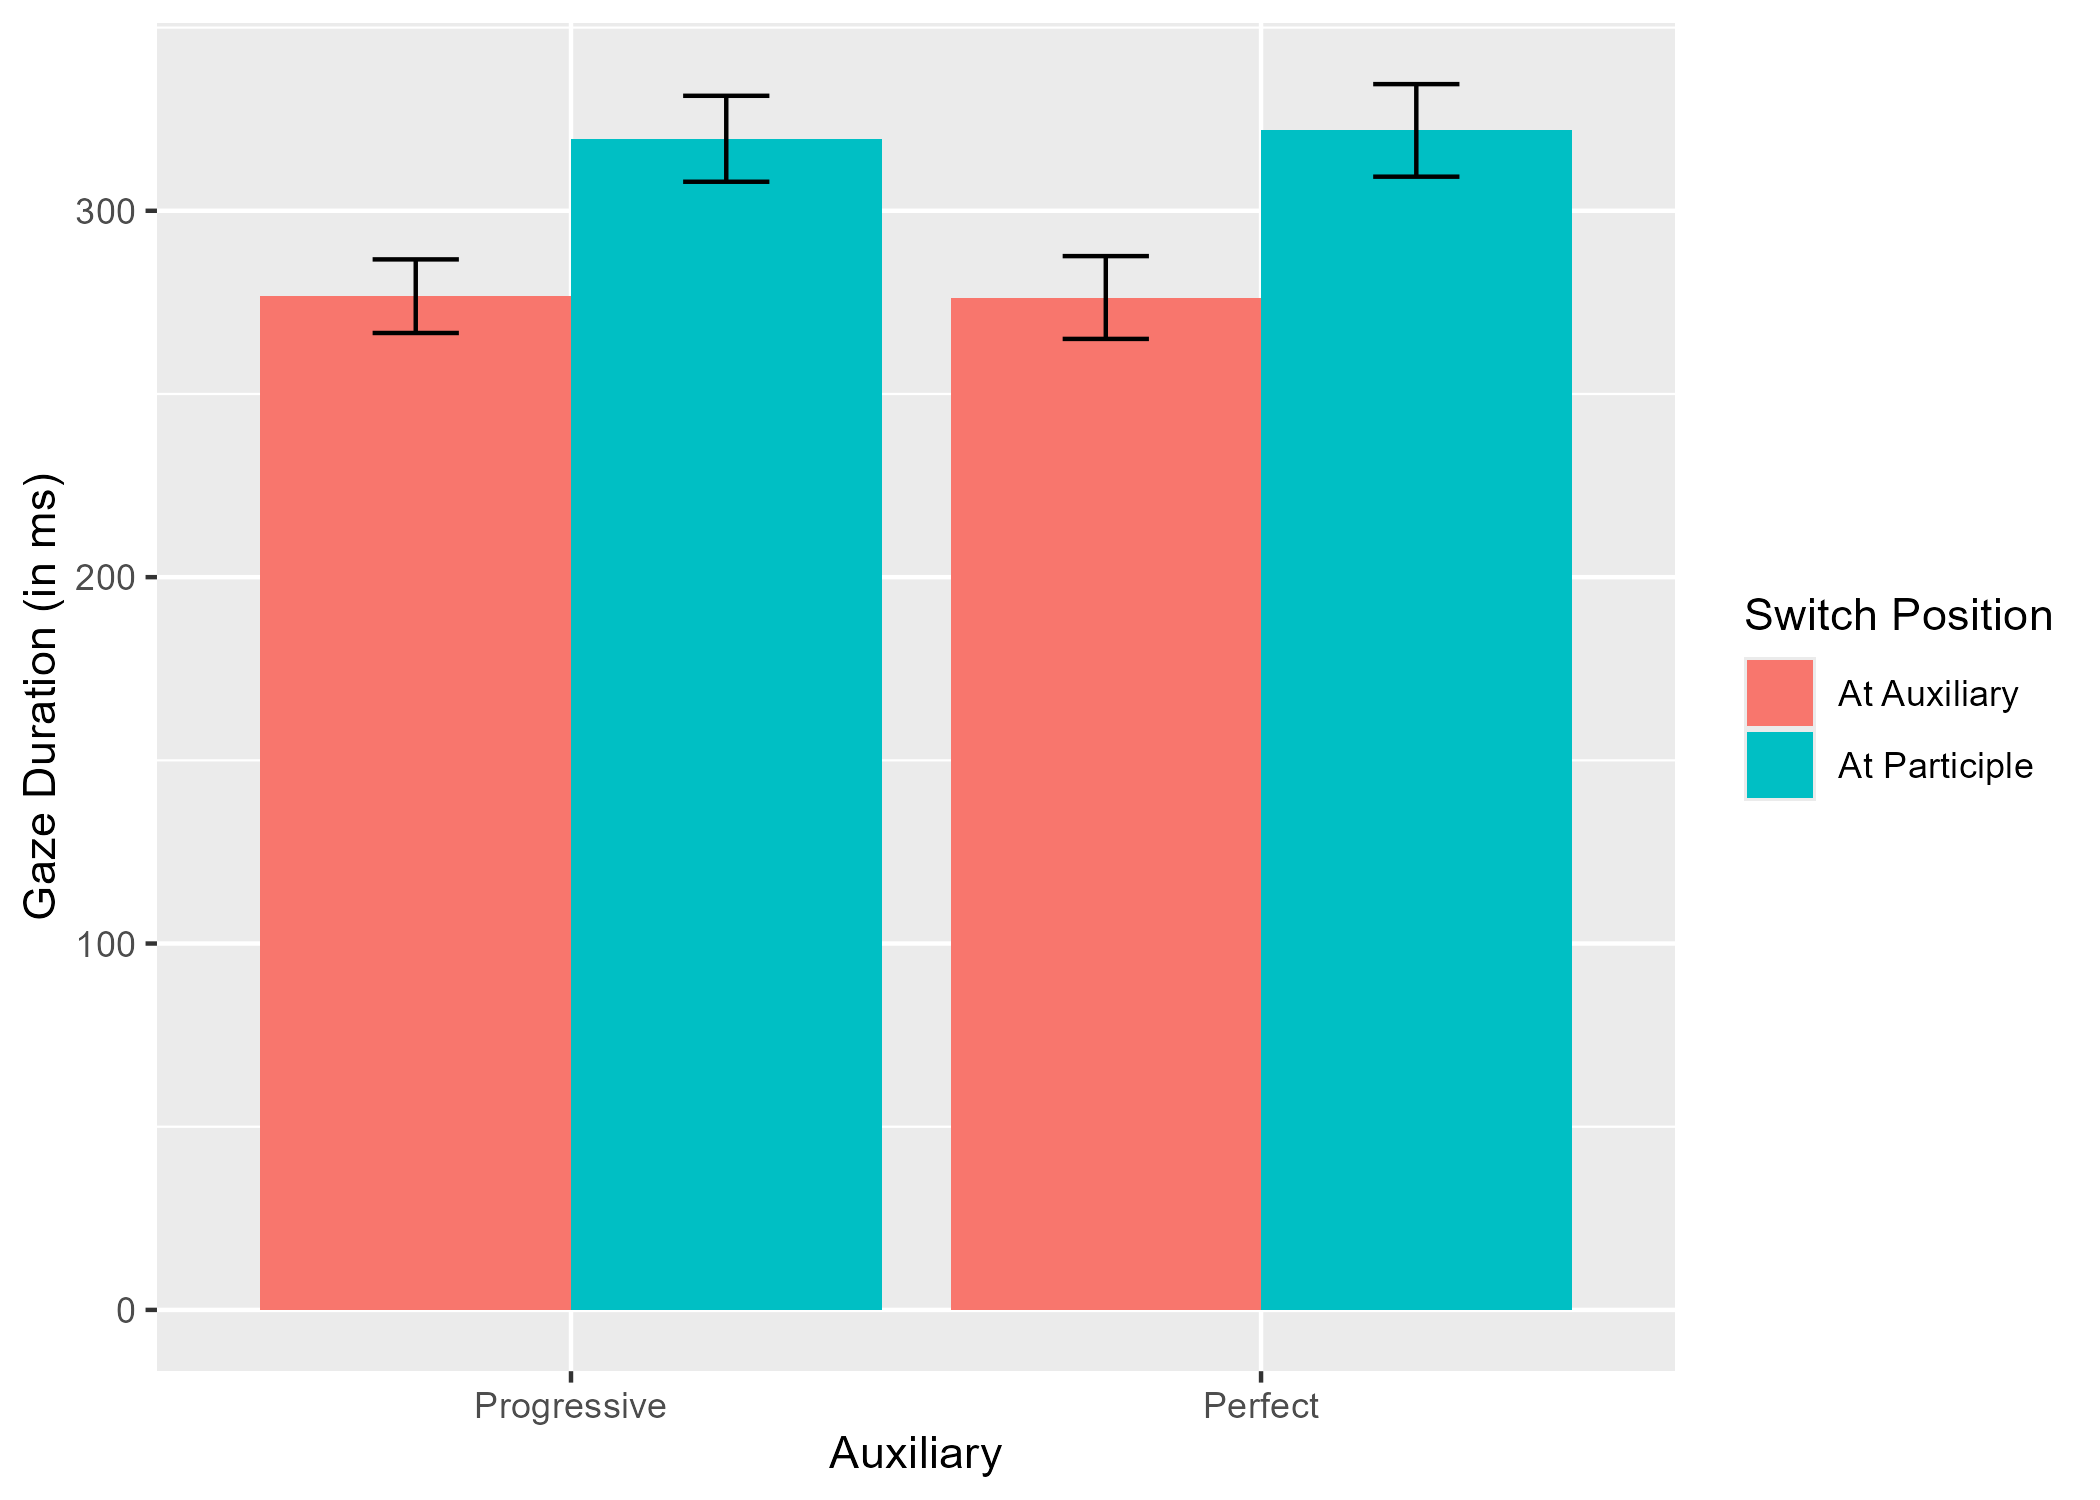
\includegraphics[height=.4\textheight]{figures/Word8_Comp_GD_Means_revisions.png}
 \caption{Mean gaze duration reading time in milliseconds on the critical region, the participle, graphed by Auxiliary Type and Switch Position. Error bars represent standard error of the mean. }
\label{fig:W8CompGD}
\end{figure}

\begin{figure}
% \includegraphics[width=\textwidth]{figures/Figure 2.1.png}
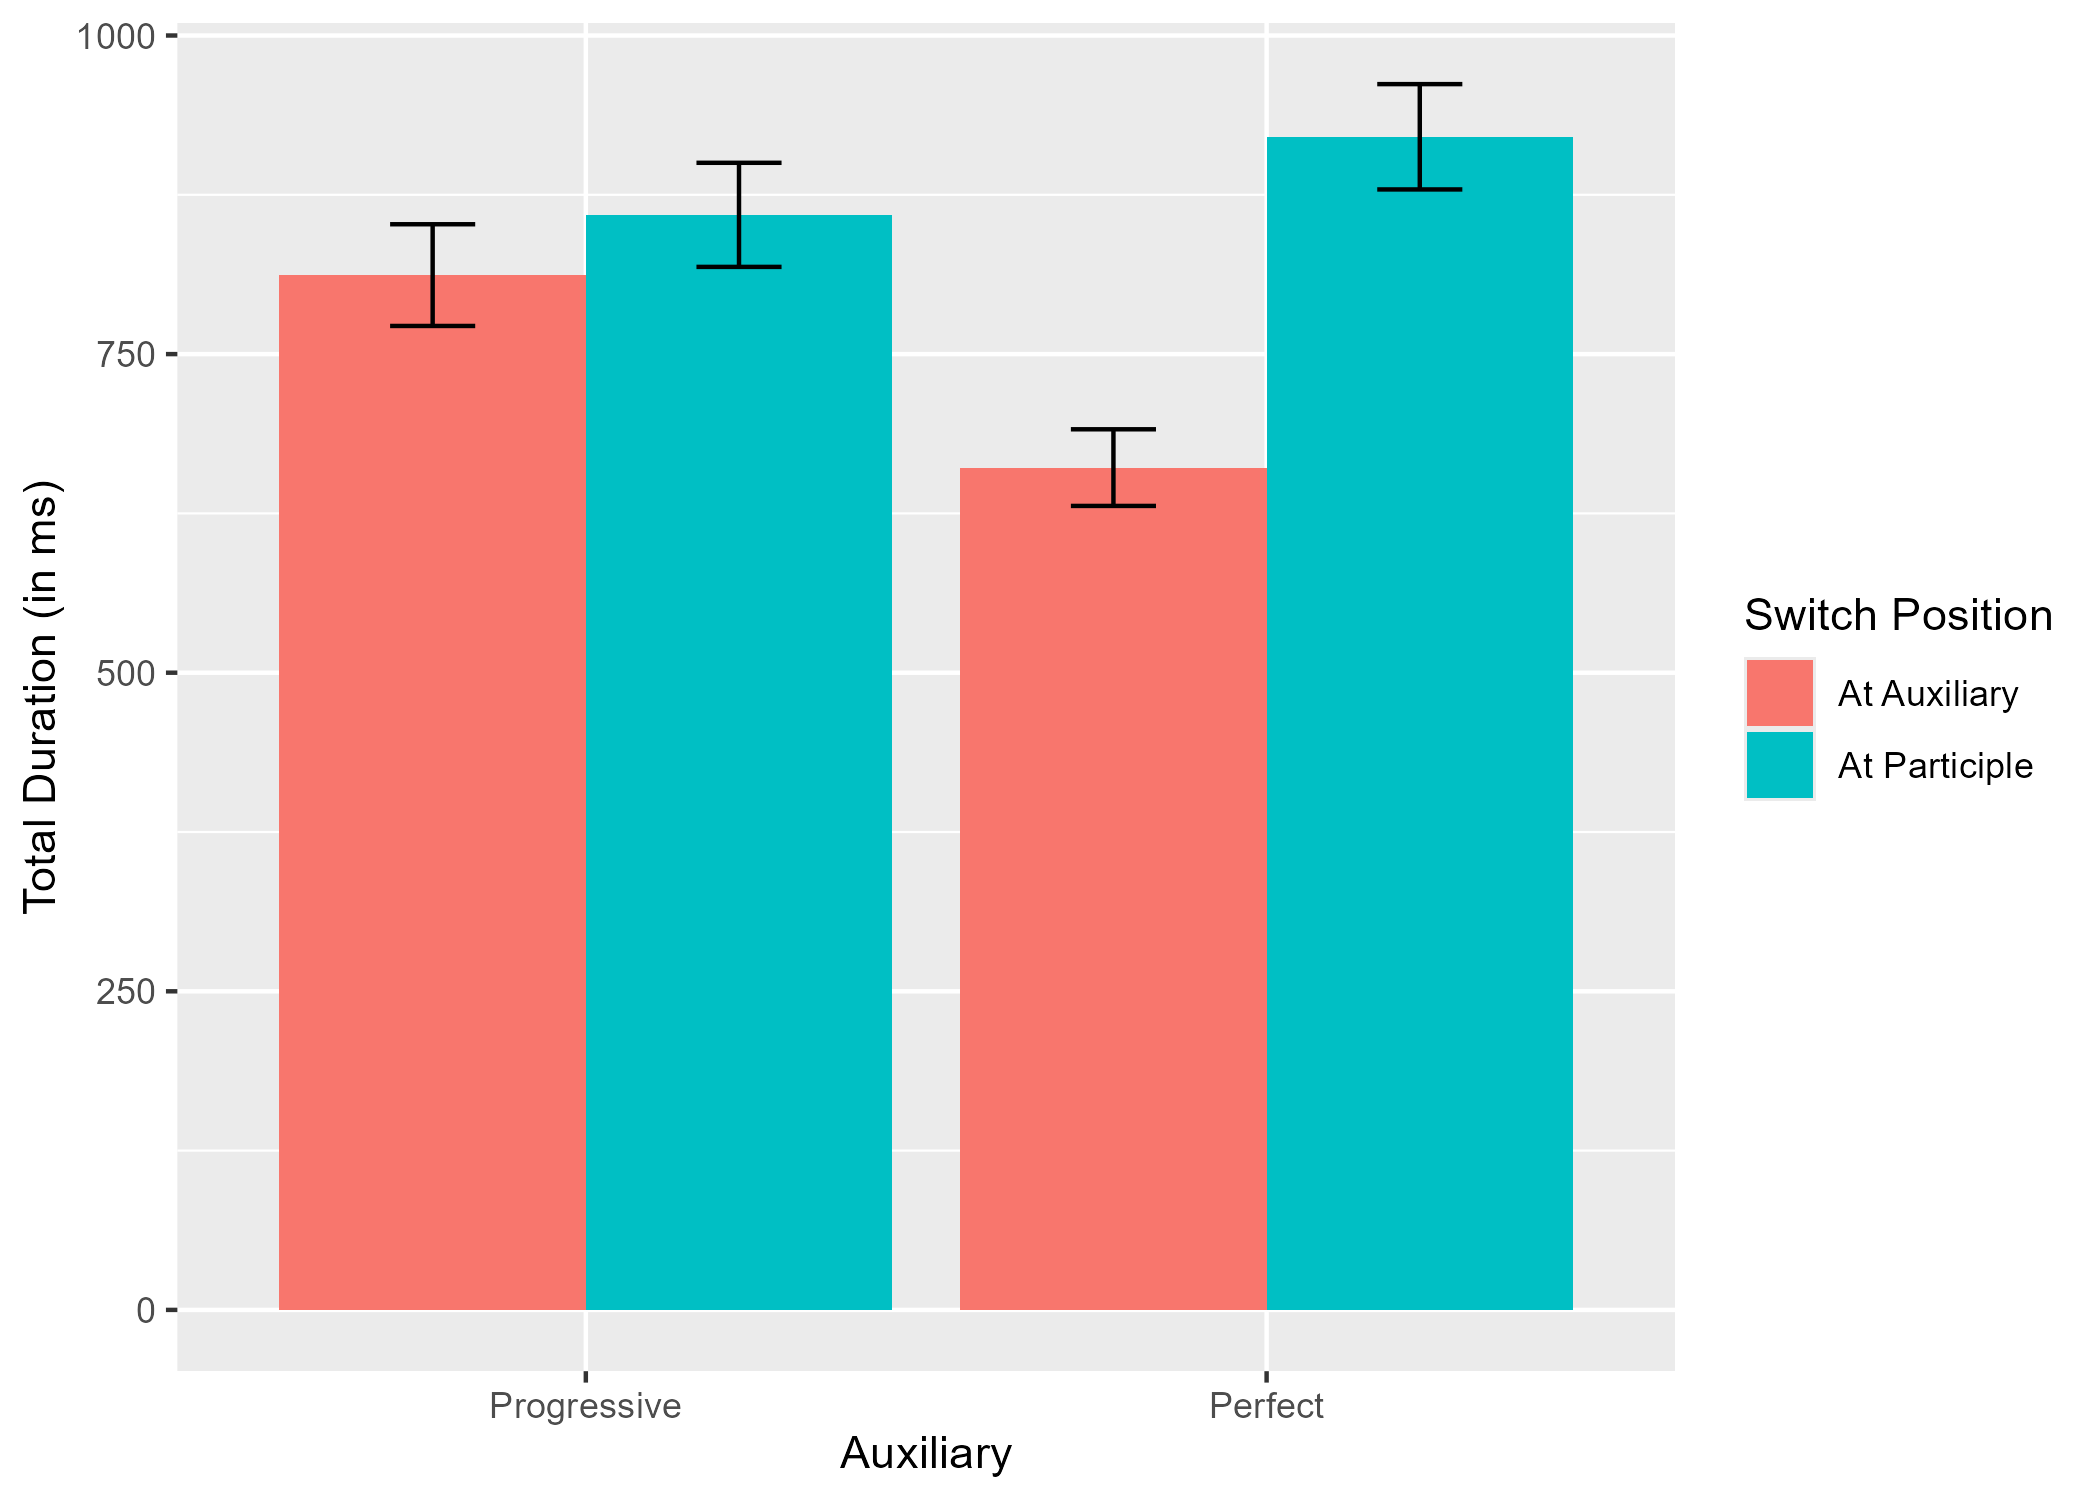
\includegraphics[height=.4\textheight]{figures/Word8_Comp_TD_Means_revisions.png}
 \caption{Mean total duration reading time in milliseconds on the critical region, the participle, graphed by Auxiliary Type and Switch Position. Error bars represent standard error of the mean. }
\label{fig:W8CompTD}
\end{figure}

\subsubsection{Spillover region (Words 9 and 10)}
On the gaze duration dataset, the linear mixed-effects model had a random effects structure that only included random intercepts on Participants and Items. This model did not reveal any interaction or main effects (all $p > 0.48$).

However, the model fit for the total duration dataset indicates a significant finding. This model had a random effects structure that includes random intercepts and slopes for Switch Position and Auxiliary (no interaction) on Participants and random intercepts on Items. The interaction between Switch Position and Auxiliary was significant ($b = 162.6, SE = 53.73, df = 228.48, t = 3.026, p = 0.003$). None of the main effects were significant (all $p > .137$). We conducted pairwise tests on the interaction and as before, two contrasts were significant: the contrast between perfect auxiliary codeswitches in which switches at the participle were significantly slower than switches at the auxiliary (difference $= 112.2, SE = 39.4, df = 102, t =  2.848, p = 0.027$) as well as the contrast between the switch at participle trials with switches involving the progressive being read faster than those involving the perfect (difference $= 126.8, SE = 40.6, df = 87.9, t = 3.121, p = 0.013$). As only the model for total duration shows a significant finding, we present a graph only for those results in Figure \ref{fig:W9_10CompTD}.

\begin{figure}[t]
% \includegraphics[width=\textwidth]{figures/Figure 2.1.png}
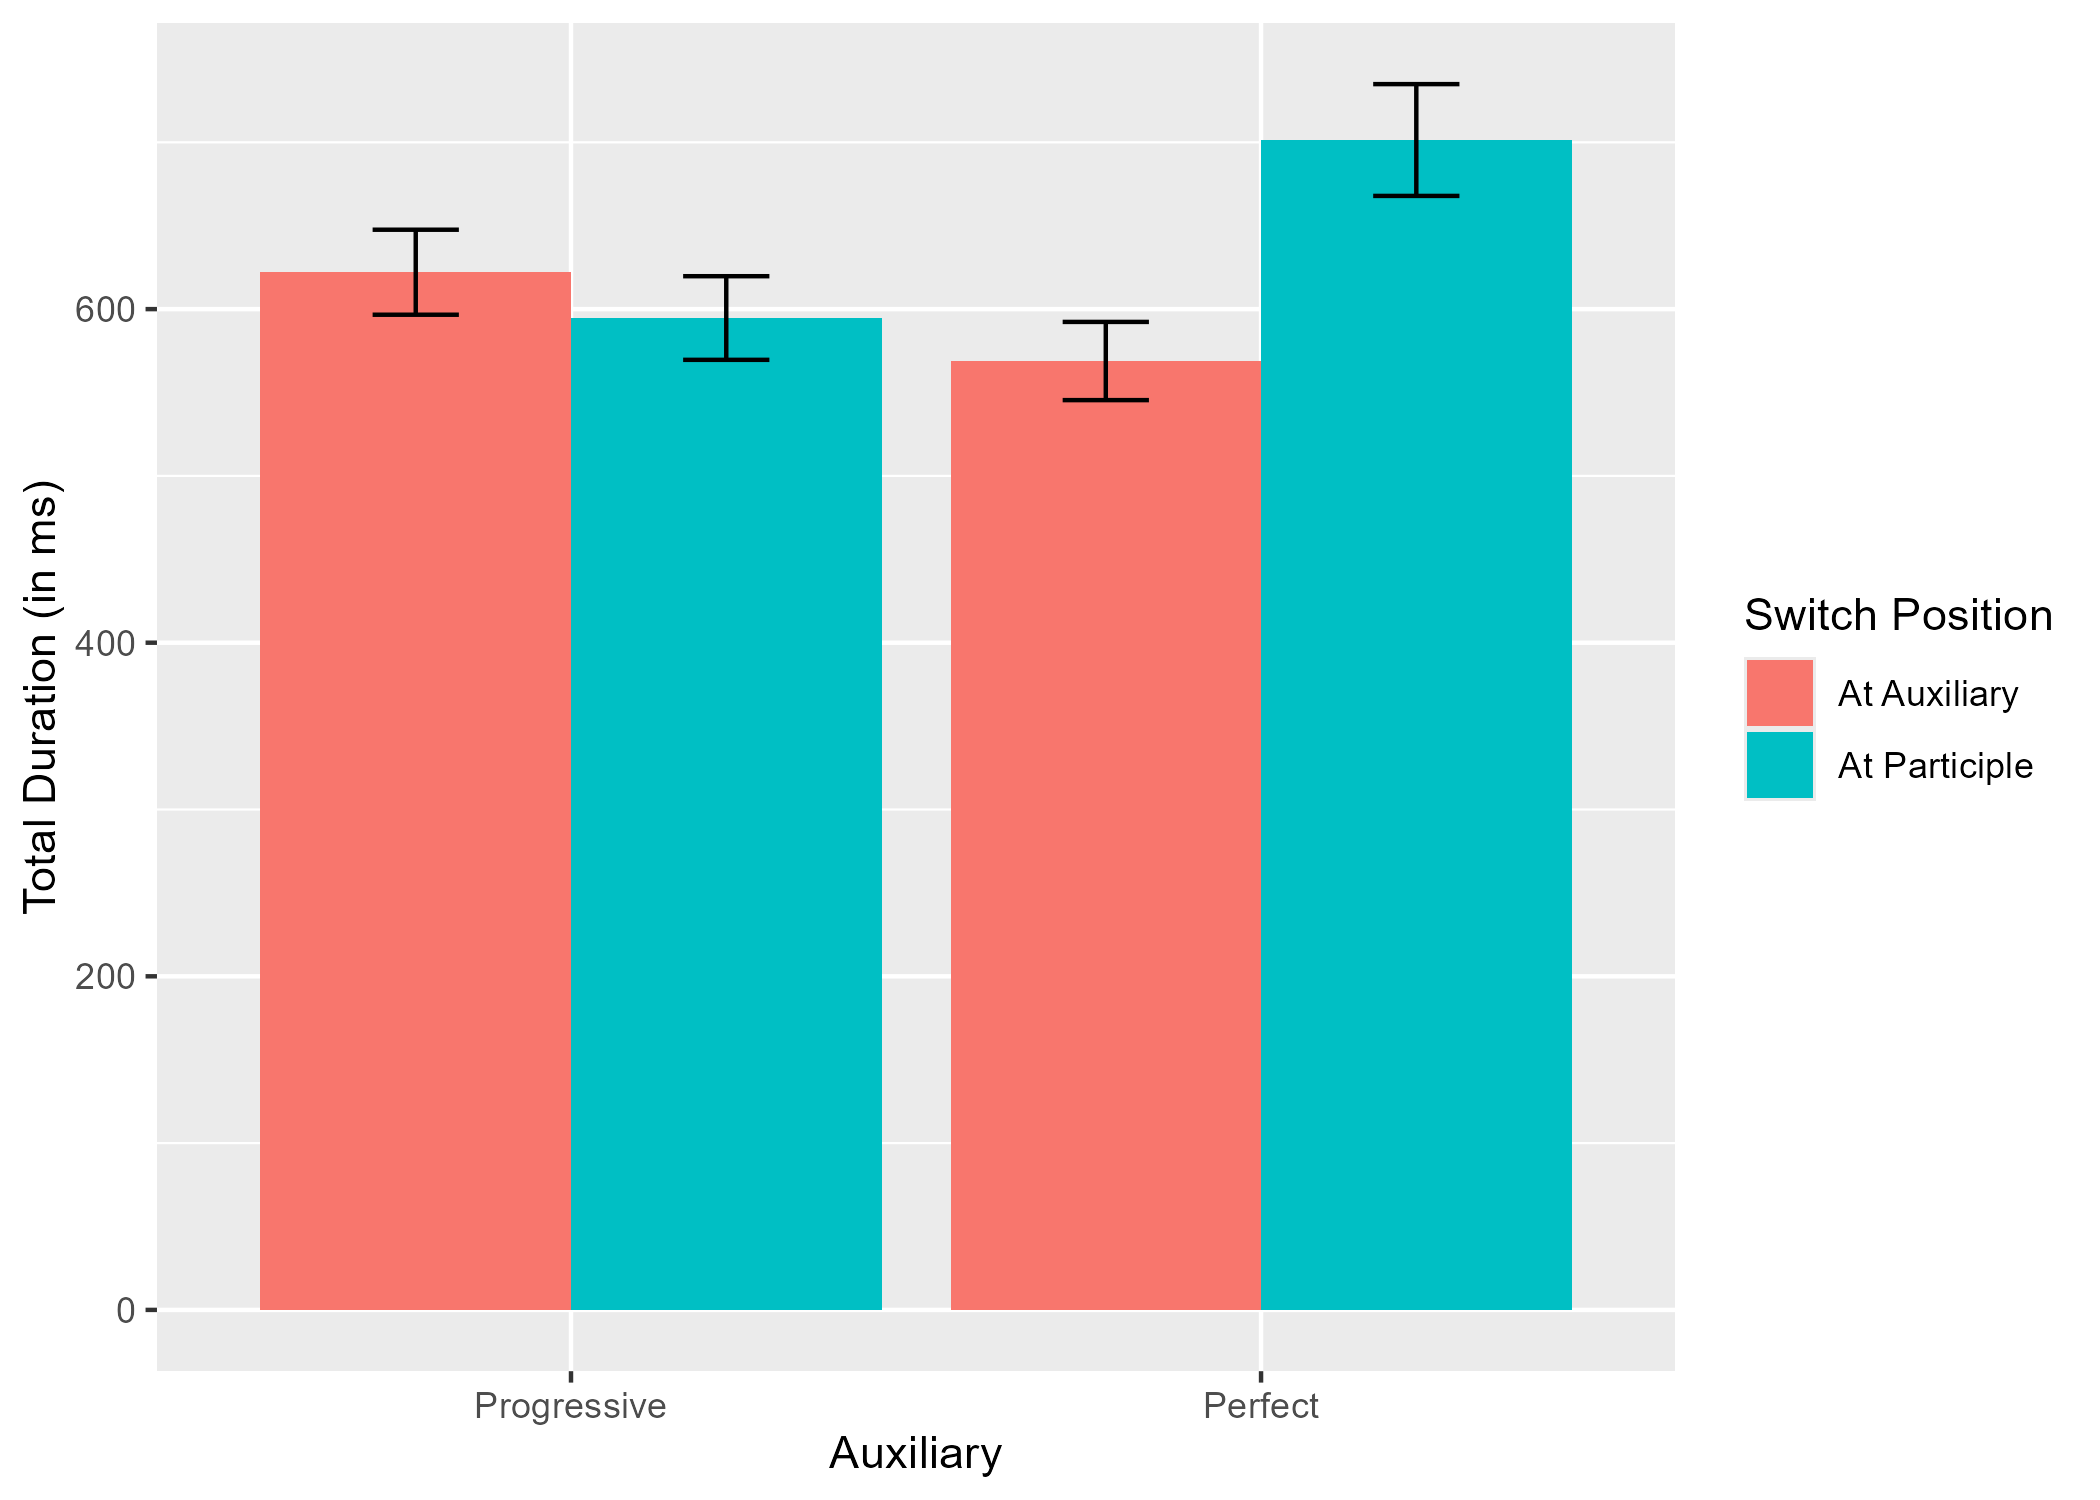
\includegraphics[height=.4\textheight]{figures/Word9_10_Comp_TD_Means_revisions.png}
 \caption{Mean total duration reading time in milliseconds on the spillover region (Words 9 and 10) following the critical participle region graphed by Auxiliary Type and Switch Position. Error bars represent standard error of the mean.}
\label{fig:W9_10CompTD}
\end{figure}

To summarize, on the critical word region (i.e., the participle), L2 Spanish readers tasked with completing a comprehension question showed sensitivity to switch position in the early reading measure of gaze duration, reading switches at the participle more slowly than at the auxiliary irrespective of auxiliary. In the later reading measure of total duration, these L2 participants demonstrated a differential sensitivity to switch position based on the auxiliary. The participants showed no difference in reading times across switch position for the codeswitches that include the progressive auxiliary, \textit{estar}. However, for codeswitches that include the perfect auxiliary, \textit{haber}, L2 Spanish participants read the codeswitches at the participle more slowly than at the auxiliary. This finding mirrors that of early Spanish-English bilinguals and L2 English participants and is consonant with the production asymmetry found in the immediate bilingual environment of these participants. We turn now to the results for the L2 Spanish group that completed a forced-choice grammaticality judgment task.

\subsection{Grammaticality judgment group analysis}
For the group that completed grammaticality judgments, we only removed trials on which reading measures were below 150 ms as the grammaticality of these trials does not have a clear target, especially codeswitches with the perfect auxiliary that switch at the participle. This data trimming procedure resulted in a reduction of 56\% of the dataset for gaze duration and 49\% of the dataset for total duration. For the spillover region, data trimming resulted in a loss of 53\% of the dataset for gaze duration and 49\% for total duration. Immediately, we observe that the reading patterns for this group are considerably different than for the participants who completed the comprehension question task. This difference is not attributable to proficiency (self-reported or assessment based), age of acquisition, or immersive differences as noted by the descriptive statistics reported in Table \ref{tab:myname:demo}.

\subsubsection{Critical word region (Word 8)}
We fit a linear mixed-effects regression model for the gaze duration dataset including random intercepts for Participants. This model showed a significant main effect for Switch Position ($b = 113.62, SE = 17.96, df = 426.06, t = 6.327, p < 0.001$), a marginal effect for the Auxiliary ($b = 30.56, SE = 18.17, df = 430.16, t = 1.682, p = 0.093$), and a significant interaction between the two factors ($b = 71.47, SE = 36.3, df = 431.34, t = 1.969, p = 0.05$). The positive coefficients for the variable of Switch Position and Auxiliary indicate that participants read codeswitches that occurred at the participle more slowly as well as a trend towards reading the code-switches involving the perfect auxiliary, \textit{haber}, more slowly. To follow up on the interaction, we conducted pairwise tests and found several contrasting pairs that were significant. For simplification, we focus on pairs of theoretical interest from the factorial design. Comparing the switch position for each auxiliary, participants were slower to read when code-switches occurred at the participle as compared to switches at the auxiliary (for progressive \textit{estar} trials: difference $= 77.89, SE = 20.3, df = 423, t = 3.839, p = 0.001$; for perfect \textit{haber} trials: difference $= 149.35, SE = 30.2, df = 436, t = -4.944, p < 0.001$). Neither of the contrasts comparing between auxiliary structures but at the same code-switch position was significant (all $p > 0.133$).

The linear mixed-effects model that converged for total duration included random intercepts for Participants. The model output revealed a main effect for Switch Position ($b = 332.91, SE = 64.15, df = 488.84, t = 5.189, p < 0.001$), for Auxiliary ($b = 147.1, SE = 65.36, df = 491, t = 2.25, p = 0.025$), and a marginal interaction between the two factors ($b = 249.44, SE = 131.09, df = 491.14, t = 1.903, p = 0.058$). While the interaction was marginal, we decided to conduct pairwise tests to explore this trending interaction further. As above, there were several contrasts that were significant, but we report on only pairs that were theoretically of interest according to our factorial design. Reflecting the main effect of Switch Position, participants read the critical region more slowly when code-switches occurred at the participle (for progressive \textit{estar} trials, difference $= 208.2, SE = 69.8, df = 478, t = 2.982, p = 0.016$; for perfect \textit{haber} trials, difference $= 457.6, SE = 110, df = 498, t = 4.158, p < 0.001$). When comparing across auxiliaries for code-switches occurring at the same syntactic juncture, only the contrast for code-switches at the participle was marginally significant, with the perfect condition being slower than the progressive condition (difference $= 271.8, SE = 112, df = 499, t = 2.428, p = 0.073$). Graphs for both reading measures on the critical region are provided in Figures \ref{fig:W8_GrammGD} and \ref{fig:W8_GrammTD}.

\begin{figure}
% \includegraphics[width=\textwidth]{figures/Figure 2.1.png}
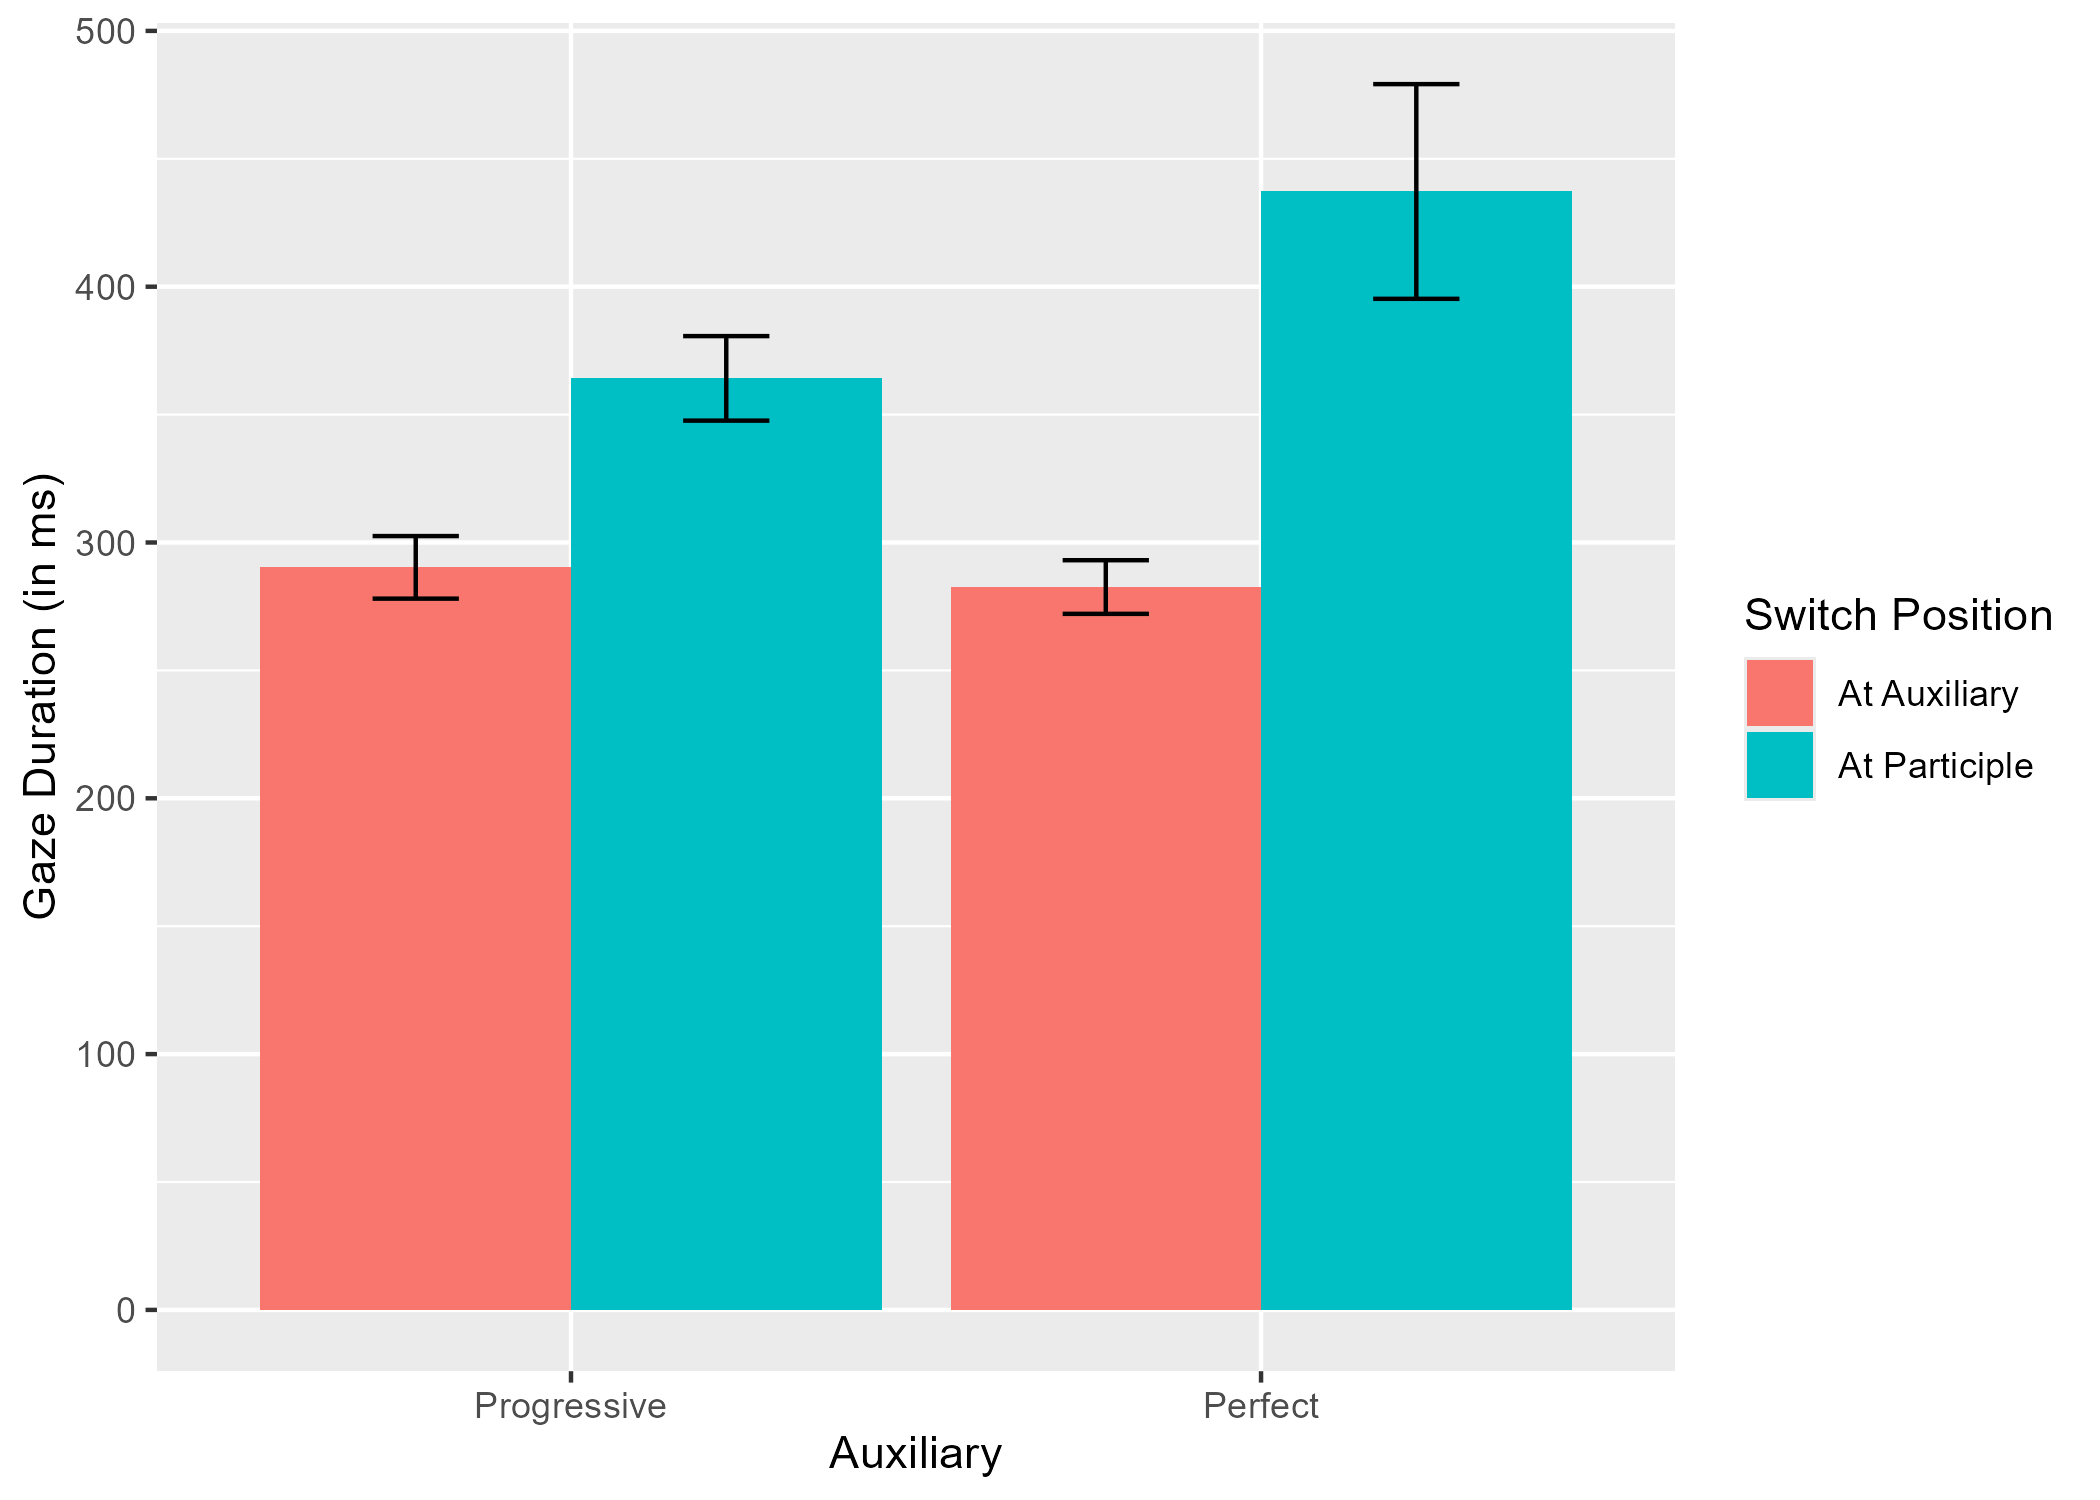
\includegraphics[height=.4\textheight]{figures/Word8_gramm_GD_Means_revisions.png}
 \caption{Mean gaze duration reading time in milliseconds on the participle critical region graphed by Auxiliary Type and Switch Position. Error bars represent standard error of the mean.}
\label{fig:W8_GrammGD}
\end{figure}

\begin{figure}
% \includegraphics[width=\textwidth]{figures/Figure 2.1.png}
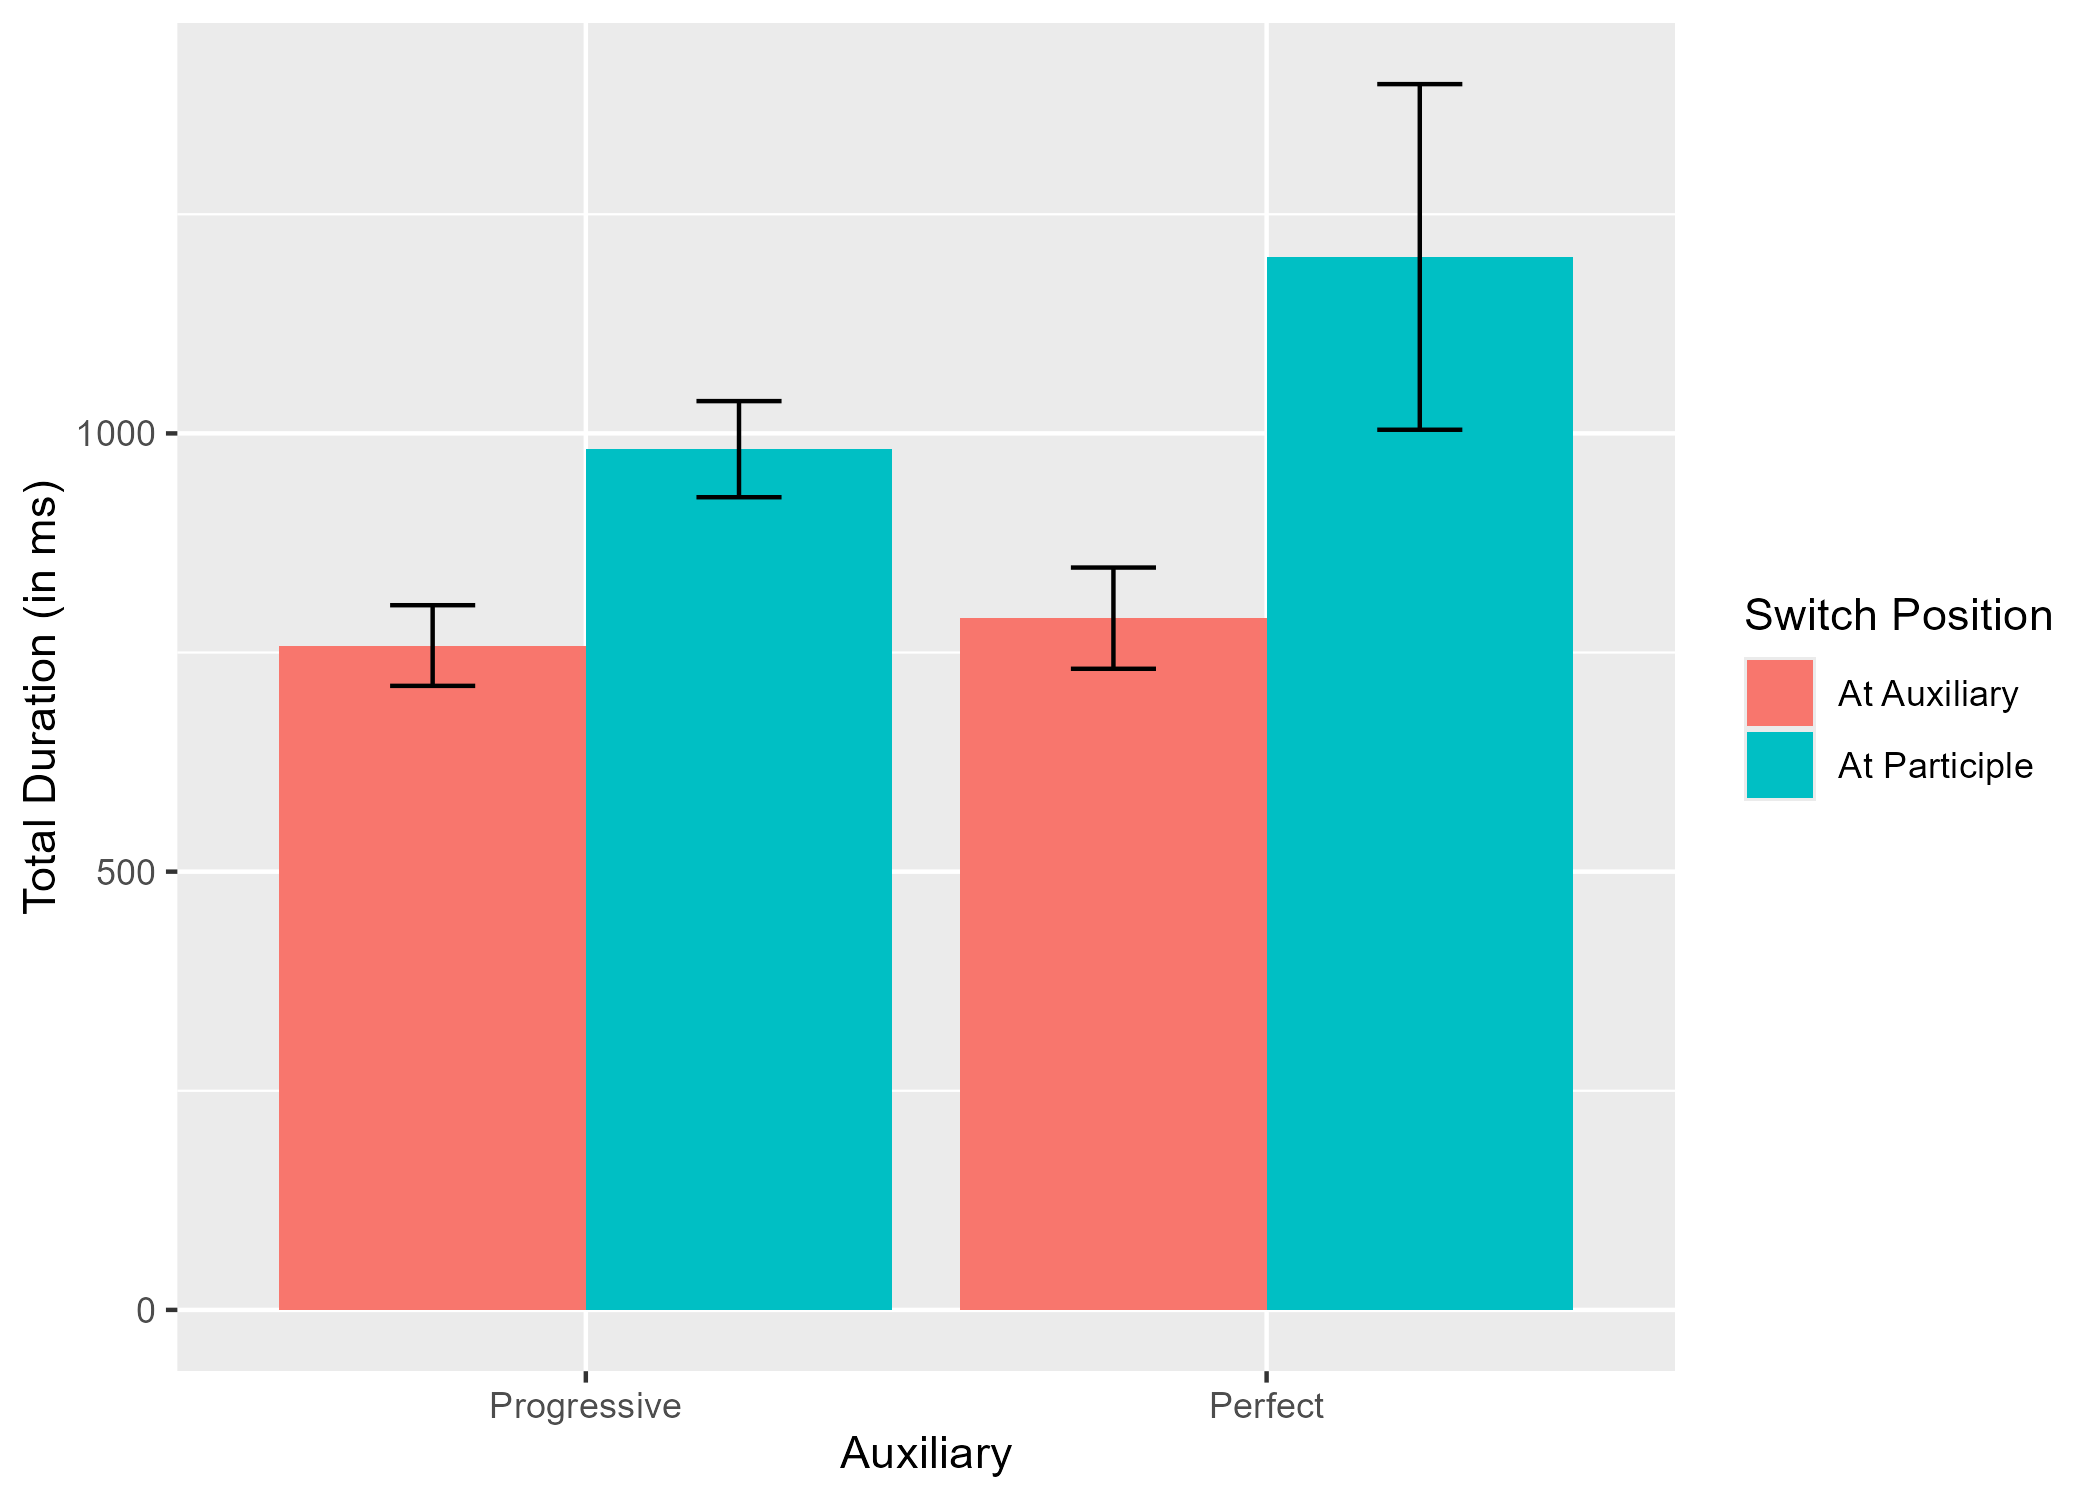
\includegraphics[height=.4\textheight]{figures/Word8_gramm_TD_Means_revisions.png}
 \caption{Mean total duration reading time in milliseconds on the participle critical region graphed by Auxiliary Type and Switch Position. Error bars represent standard error of the mean.}
\label{fig:W8_GrammTD}
\end{figure}

\subsubsection{Spillover region (Words 9 and 10)}
In the spillover region, the linear mixed-effects regression model fit for gaze duration included a random effects structure with random intercepts on Participants and Items. This model revealed a significant effect of Switch Position ($b = 32.9, SE = 15.54, df = 314.23, t = 2.116, p = 0.035$). No effect for Auxiliary or interaction was found (Auxiliary: $b = 25.93, SE = 15.79, df = 323.77, t = 1.642, p = 0.102$; interaction: $b = 47.39, SE = 31.65, df = 312.91, t = 1.5, p = 0.135$). As in the critical region, the main effect of Switch Position indicates slower reading on trials where the code-switch occurs at the participle. Note, however, that visually, the effect seems to largely be attributable to the magnitude difference in the \textit{haber} trials (mean difference $= 74.67$) rather than the difference in the \textit{estar} trials (mean difference $= 0.91$), despite the lack of evidence for a significant interaction.

The model for total duration had the same random effects structure as for gaze duration. This model also only detected a significant main effect for Switch Position ($b = 129.53, SE = 50.27, df = 369.47, t = 2.576, p = 0.01$). There was no significant effect for Auxiliary or the interaction between both factors (Auxiliary: $b = 79.39, SE = 51.47, df = 379.5, t = 1.543, p = 0.124$; interaction: $b = 19.16, SE = 103.09, df = 372.42, t = 0.186, p = 0.853$).
Graphs visually representing the results in the spillover region are presented in Figures \ref{fig:W9_10_GrammGD} and \ref{fig:W9_10_GrammTD}.

\begin{figure}
% \includegraphics[width=\textwidth]{figures/Figure 2.1.png}
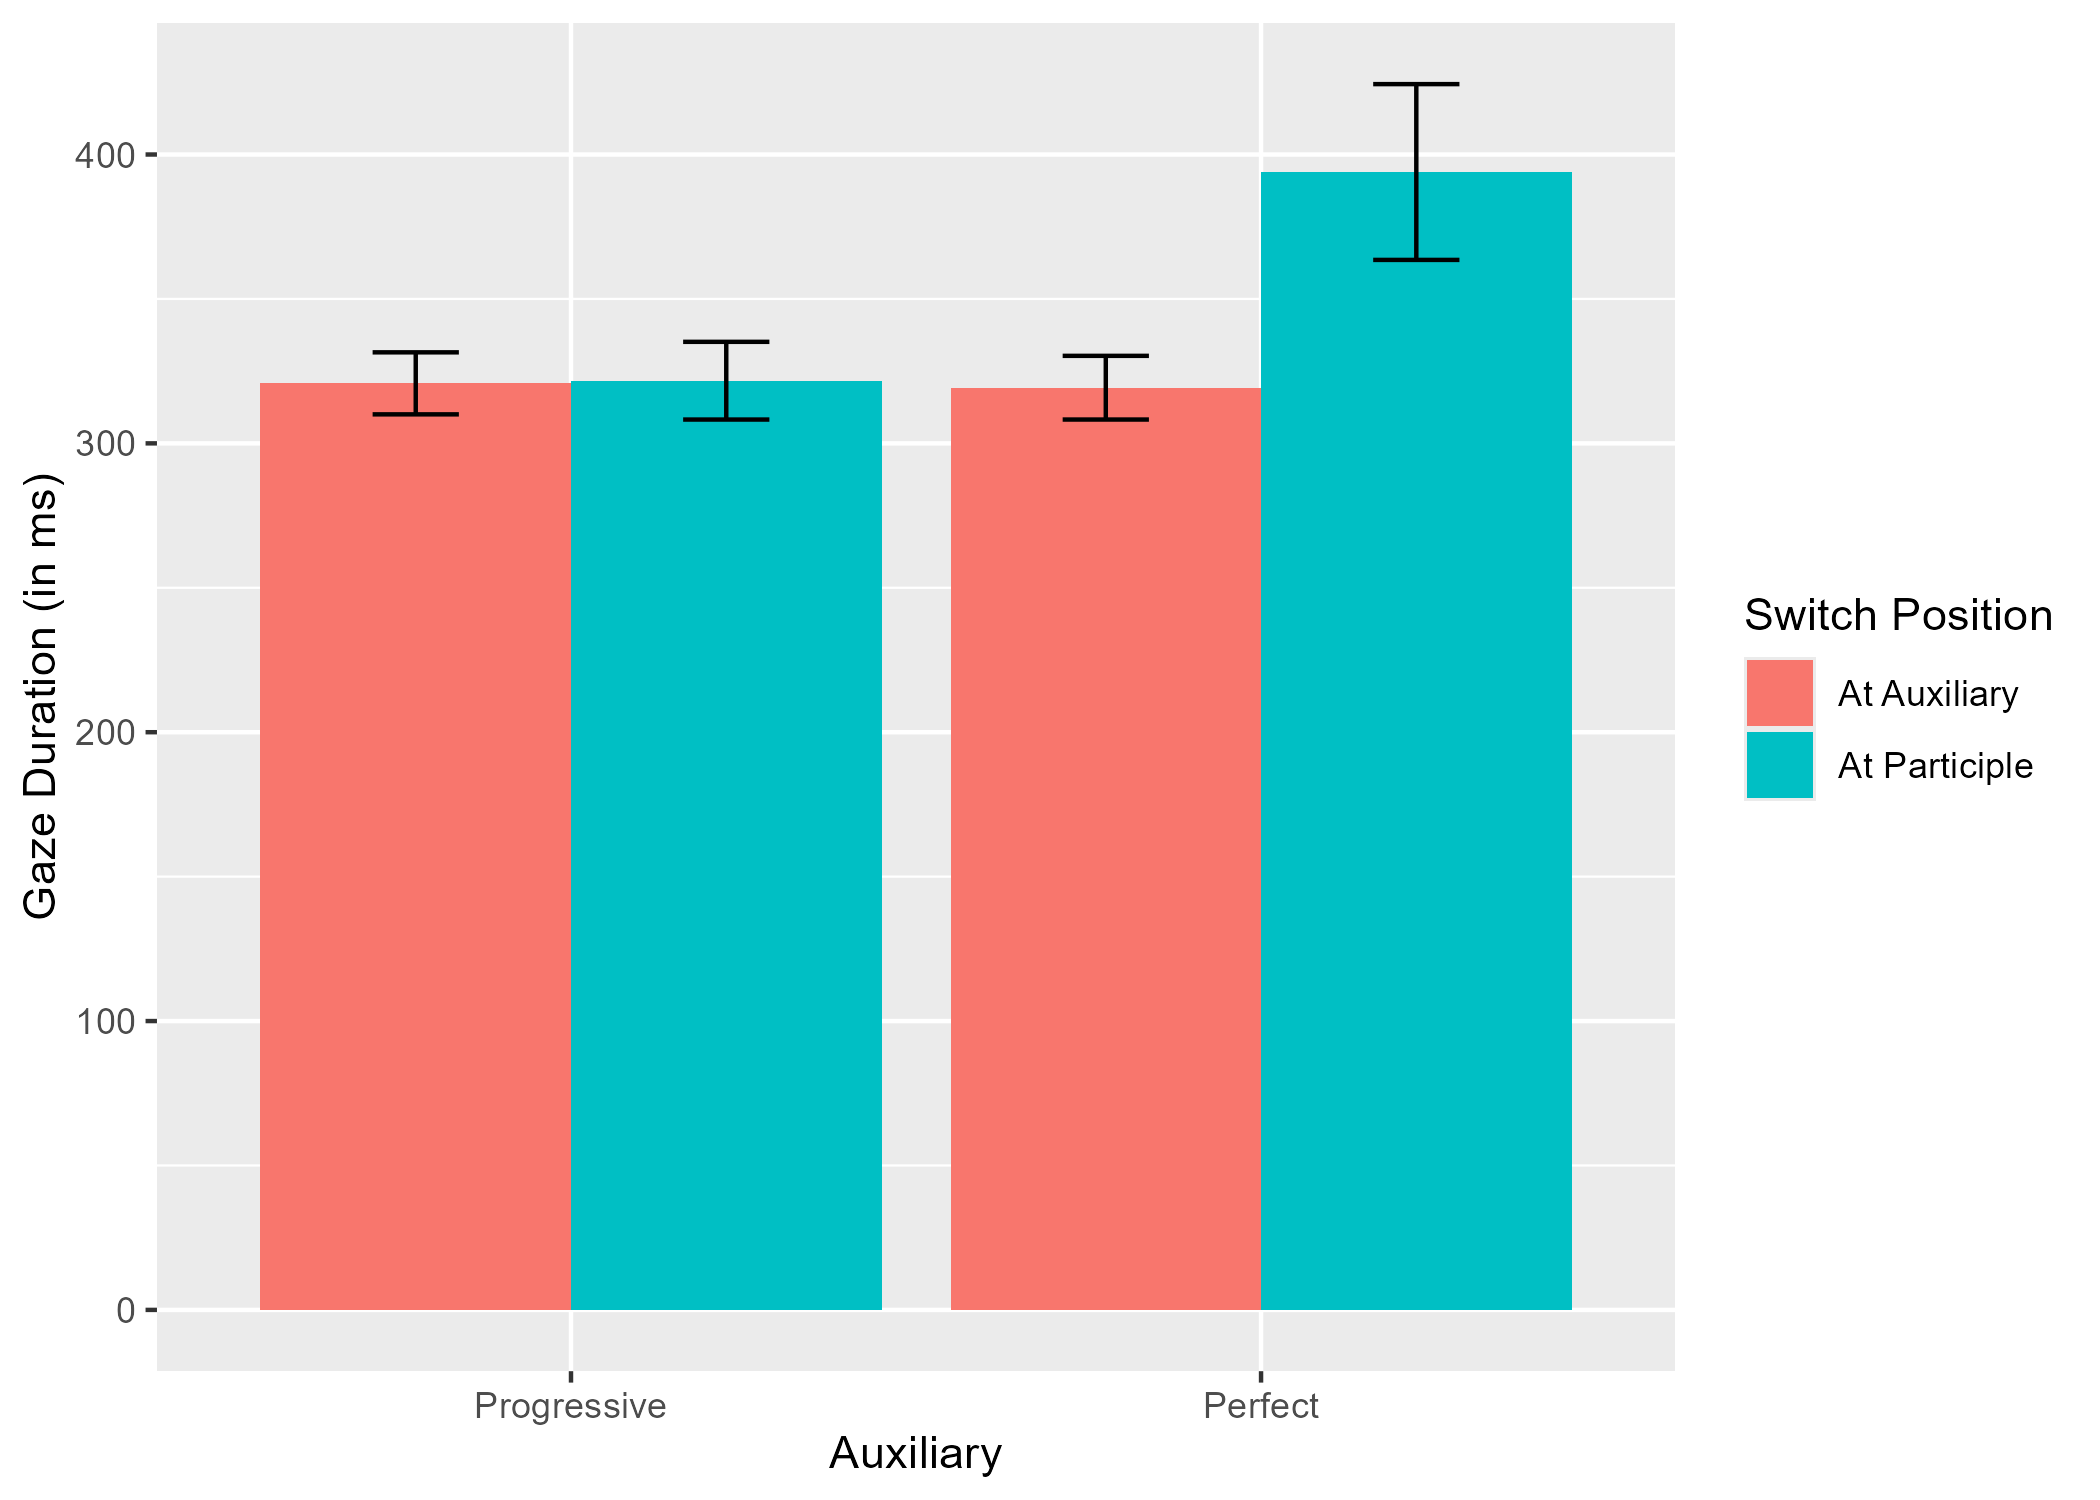
\includegraphics[height=.4\textheight]{figures/Word9_10_Gramm_GD_Means_revisions.png}
 \caption{Mean gaze duration reading time in milliseconds on the spillover region (Words 9 and 10) graphed by Auxiliary Type and Switch Position. Error bars represent standard error of the mean.}
\label{fig:W9_10_GrammGD}
\end{figure}

\begin{figure}[t]
% \includegraphics[width=\textwidth]{figures/Figure 2.1.png}
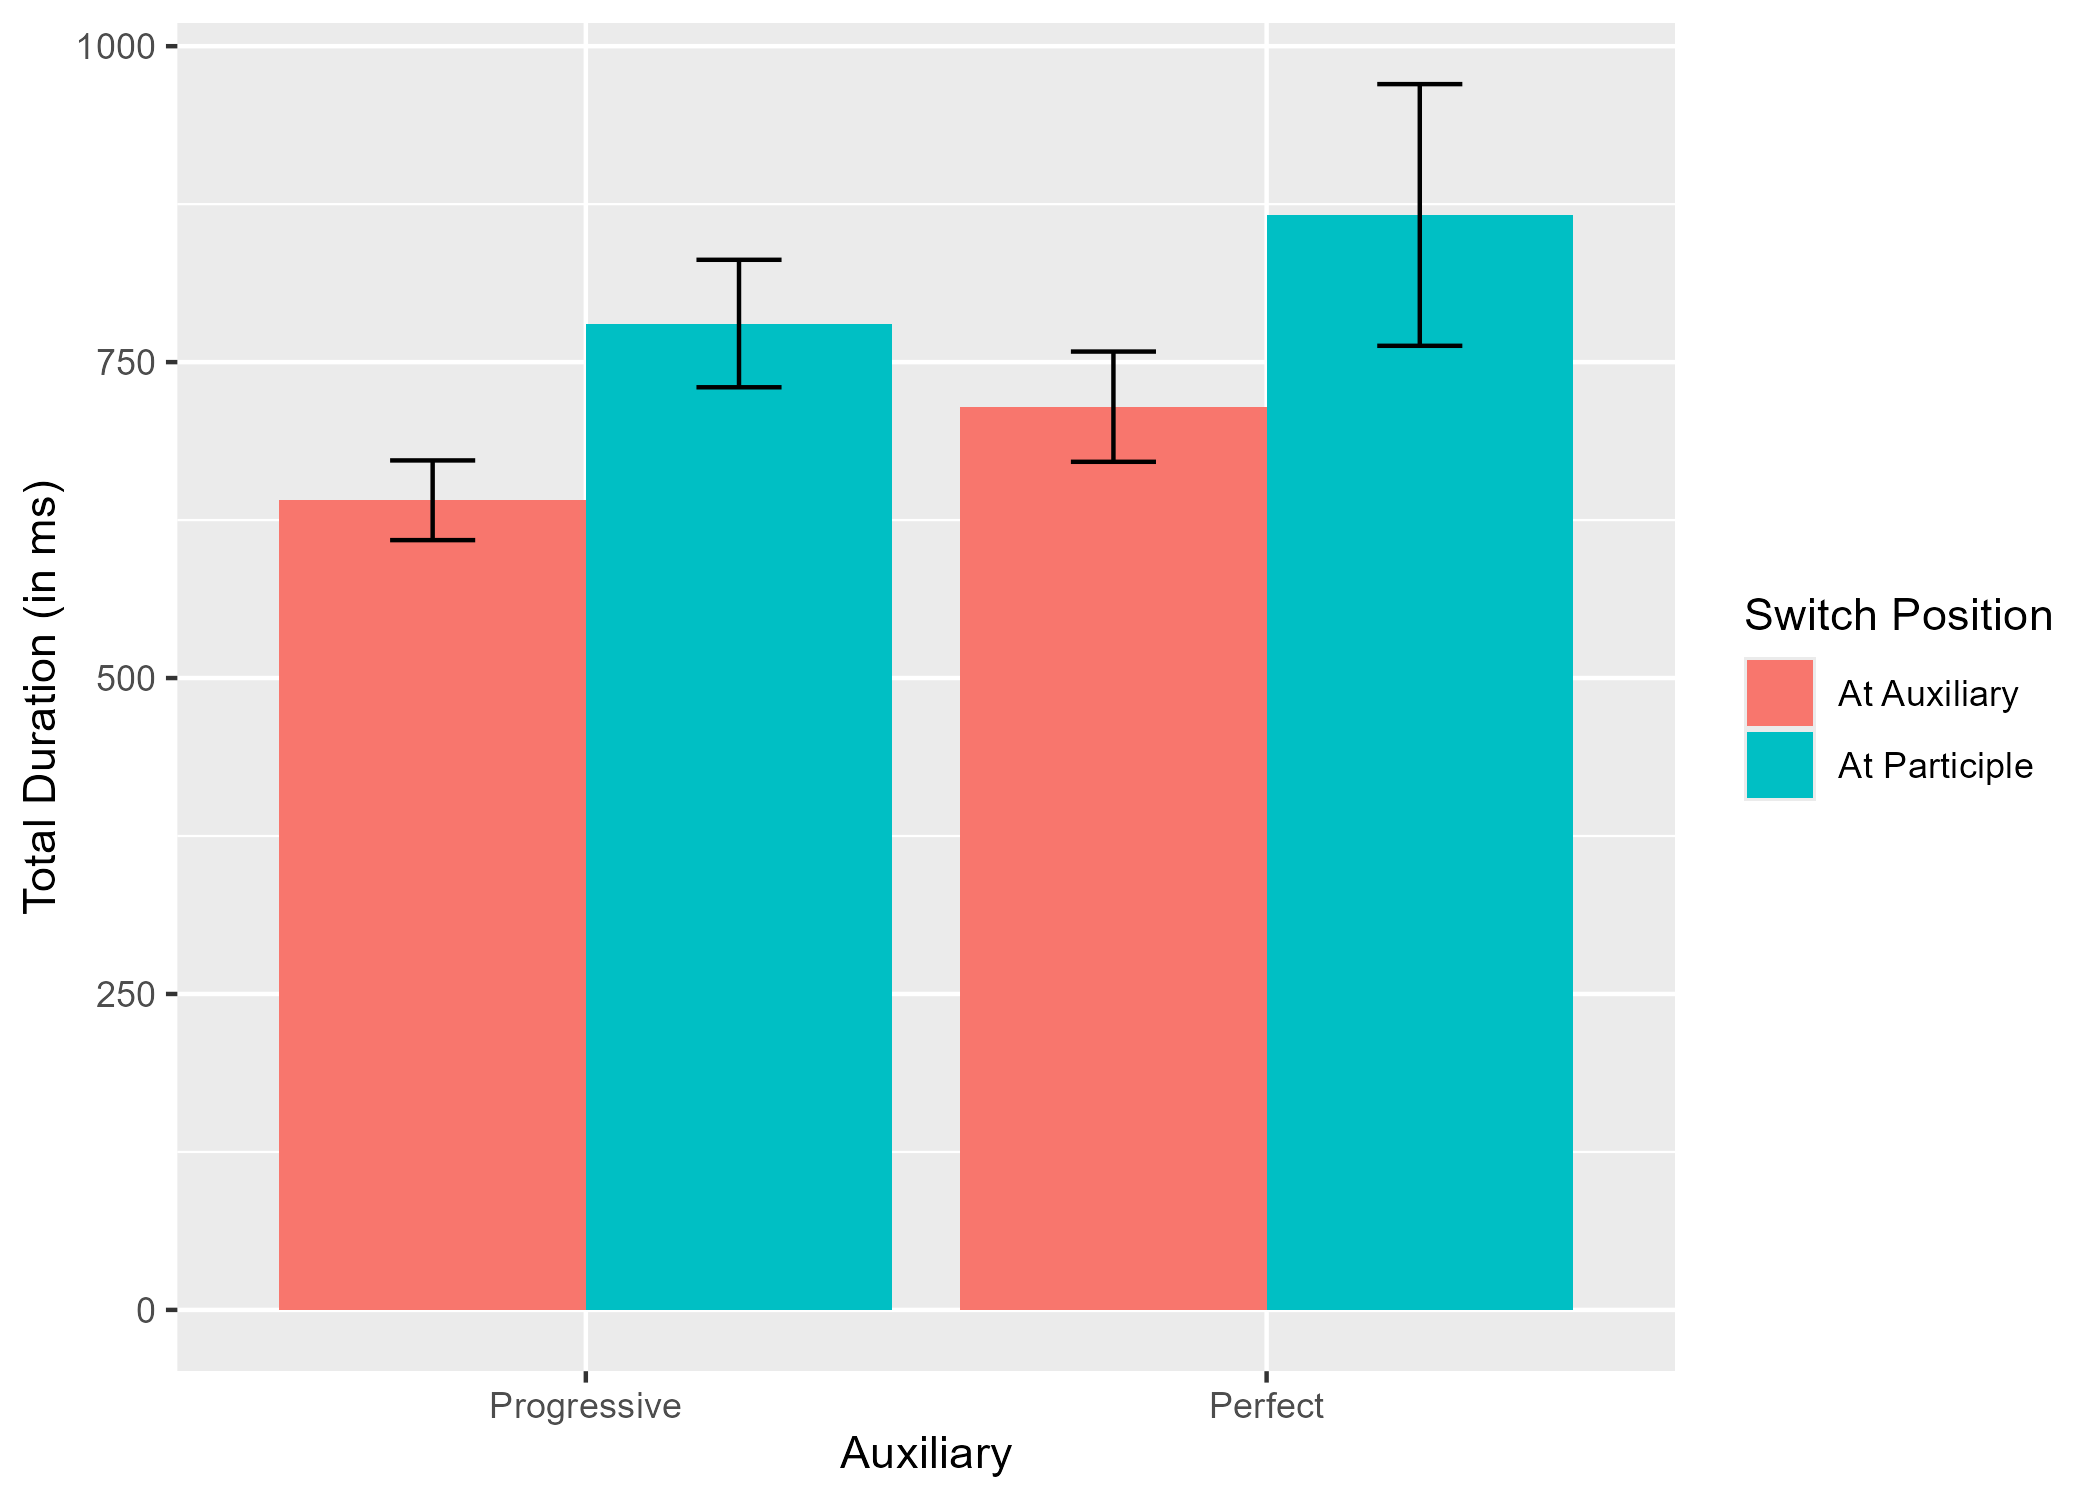
\includegraphics[height=.4\textheight]{figures/Word9_10_Gramm_TD_Means_revisions.png}
 \caption{Mean total duration reading time in milliseconds on the spillover region (Words 9 and 10) graphed by Auxiliary Type and Switch Position. Error bars represent standard error of the mean.}
\label{fig:W9_10_GrammTD}
\end{figure}

In summary, a differential reading pattern emerges for the L2 Spanish group that performed a grammaticality judgment task while reading code-switched sentences. For one, this group experienced greater data loss when trimming for fixations that were not at least 150 ms. More importantly, the only consistent finding was for Switch Position, where overall trials on which switches occurred at the participle were read more slowly than at the auxiliary. Potentially, a weak asymmetry was found in the early reading measure whereby for codeswitches occurring at the participle, the difference between the perfect conditions was greater than for the difference between the progressive conditions. However, a significant interaction between the variables of auxiliary and switch position was not found, indicating no clear differential sensitivity to codeswitch trials based on the auxiliary. These results stand in contrast to the other L2 group as well as to prior reported findings.

\section{Discussion and conclusions}
For this study, we employed eye tracking as a sensitive reading measure to investigate the real-time sentence processing of codeswitched sentences with complex verb phrases. Our participants were L2 Spanish speakers whose L1 was English and who were immersed in an environment where the use of Spanish-English codeswitching was present. Our primary objective was to investigate whether a production asymmetry attested among Spanish-English bilinguals from the same region would emerge in this L2 Spanish group. Specifically, prior findings indicated a preference for codeswitches that occur with the progressive auxiliary, \textit{estar}, thereby leading to frequent switching before and within the verb complex. In contrast, codeswitches with the perfect auxiliary, \textit{haber}, demonstrate an overwhelming preference for switching before the verb complex. This robust finding has been found in corpus studies, acceptability judgment tasks, and with eye tracking \citep{GuzzardoTamargoetal2016}.

We further investigated whether the type of behavioral task employed in experimental reading studies could influence the processing patterns of the learner group. Our results partially corroborate prior findings for Spanish-English bilinguals. Only the group that completed comprehension questions during the reading task reliably demonstrated the asymmetry in reading where perfect codeswitches that occurred at the participle were read more slowly than perfect codeswitches that occurred at the auxiliary (\textit{los estudiantes han} \textbf{borrowed} v. \textit{los estudiantes} have \textbf{borrowed}), a finding that was not as evident for the progressive codeswitches (\textit{los estudiantes est\'an} \textbf{borrowing} v. \textit{los estudiantes} are \textbf{borrowing}). For the group that completed a forced-choice grammaticality judgment task, results pointed towards a short-lived effect of a general reading slowdown for switches at the participle. Before further unpacking the results for the comprehension question group, we discuss the different processing patterns for each L2 group.

The results for the between-groups manipulation of secondary task are remarkably similar to prior work \citep{ValdesKroffetal2018}. In the prior study, early Spanish-English bilinguals and Spanish L1-English L2 bilinguals participated in a reading study with a similar experimental design to the study reported here. For that study, secondary task was a within-group manipulation, where order of session was counterbalanced. As in the study here, the anticipated asymmetric processing pattern for perfect auxiliaries only robustly emerged for the session in which comprehension questions were employed. Instead, for the forced-choice grammaticality judgment session, participants read the sentences more slowly and no longer demonstrated an asymmetry for the perfect auxiliary verb complex. The authors attributed this processing difference to the overarching task demands for each type of task. They stated that the grammaticality judgment task induced metalinguistic mechanisms that differed from naturalistic sentence processing. Our findings thus align with the perspective that reading for comprehension engages naturalistic processing strategies that more closely align with production distributions found in bilingual speech communities \citep{MacizoBajo2006}.

Despite these similarities, we should point out that the participants from our study were different for each task session, although they came from the same population and were immersed in the same environment. The groups did not differ on a number of self-reported and assessment-based metrics in Spanish; however, the greater data loss for the grammaticality judgment task group was not expected, especially since data trimming only included removal of fixations that were less than 150 ms. Visual inspection of the eye-tracking data did not reveal any systematic differences in quality of the eye-tracking data (except for the one participant who was removed from analysis). Nevertheless, a replication with more participants in each session or using the within-participants design reported in \citet{ValdesKroffetal2018} would help ensure greater confidence in the overall findings. Future studies should also consider other forms of common experimental linguistic tasks such as an acceptability judgment task with a Likert scale or visual analogue scales. Analyses that include procedures from signal detection theory such as d’ could also rule out potential participant bias.

Focusing on the results for the group that completed comprehension questions during reading, we highlight two important findings in relation to prior results with early Spanish-English and L2 English bilinguals \citep{Guzzardo2013,GuzzardoTamargoetal2016}. First, our hypothesized asymmetry was found primarily for the late reading measure, total duration, and second, it extended into the spillover region. Prior work also robustly found the asymmetry with the early reading measure of gaze duration. This difference in timecourse suggests that the L2 participants had not yet automatized their sensitivity to the codeswitching patterns to which they are potentially exposed. Rather, their sensitivity emerges at later stages of reading that integrate regressions and re-reads of relevant regions. We can only speculate at this point if this timecourse difference is a hard constraint or if the L2 Spanish group will begin to show sensitivity in an early reading measure with increasing proficiency and/or exposure. While the effect only emerged in later stages of processing, it was a sustained effect, further underscoring that this purported asymmetry arises due to greater difficulty in integration of codeswitches within the mixed verb compound if they involve the perfect auxiliary.

Taken together, the processing differences between the L2 Spanish groups and the later and sustained emergence of the asymmetry in the timecourse of reading for participants engaged in naturalistic reading, lead us to attribute the processing of codeswitched structures to be driven more generally by experiential factors, including community norms. Specifically for the linguistic structures investigated in our study, this asymmetry arises from exposure to bilinguals who codeswitch and commonly switch in the verb phrase with the progressive auxiliary but not with the perfect auxiliary. While community preferences play an important role, the locus for the asymmetry likely derives from the grammatical constraints imposed by the participating languages, as we have argued elsewhere \citep{GuzzardoTamargoetal2016,ValdesKroffDussias2023}. One such explanation may be due to the further grammaticalization of the perfect auxiliary in comparison to the progressive form in Spanish. Its status as a dependent form may very well prevent or highly disfavor codeswitches between the auxiliary and the participle.

The findings for the comprehension group subsequently offer additional evidence for a connection between production distributions and sentence processing as claimed by experience-based accounts such as the Production-Distribution-Comprehension framework \citep{MacDonald2013}. This model claims that ease of sentence processing is directly related to the frequency of different structures in production found in a speaker community in combination with universal pressures on speech planning such as incorporating easier elements first in an utterance. Therefore, we do not expect bilinguals from different communities to necessarily engage in the same frequency of codeswitching patterns, a claim that is supported by corpus analysis and acceptability data across different Spanish-English communities for the structures used in our study \citep{Balam2016,Balametal2020}. One prediction that stems from these comparative differences across bilingual communities is that their processing of these structures should be quite different based on community norms, independent of proficiency, a finding that we have begun to explore \citep{Treadwayetal2025}. A comparative sentence processing approach will be necessary to offer key evidence to test our hypothesis. If other bilingual communities, such as Spanish-English bilinguals in Belize who demonstrably show frequent use of different verb phrase code-switches, nevertheless show the asymmetric sensitivity reported here, then the role of community norms and exposure would not be as important as we claim.



One prediction that stems from these comparative differences across bilingual communities is that their processing of these structures should be quite different based on community norms - independent of proficiency - a finding that we have begun to explore \citep{Treadwayetal2025}. A comparative sentence processing approach will be necessary to offer key evidence to test our hypothesis. If other bilingual communities, such as Spanish-English bilinguals in Belize who demonstrably show frequent use of different verb phrase code-switches, nevertheless show the asymmetric sensitivity reported here, then the role of community norms and exposure would not be as important as we claim. This comparative approach fundamentally depends on the availability of bilingual corpora from different communities.

% We want to emphasize that at heart we are psycholinguists who principally work with controlled and constructed stimuli and tackle questions about prediction, integration, and sentence processing in bilingual speech and text.  Nevertheless, we have been deeply influenced by the work of Margaret Deuchar and her many collaborators over the years. Our work depends on a clear understanding of the patterns of use among different bilingual communities. The care with which Margaret and her team have developed and selflessly shared publicly available corpora such as the Bangor Miami Corpus \citep{Deucharetal2014} has been fundamental to the development of our own research program. Over the years, we have been able to investigate our research questions, extend findings, and develop new frameworks for a greater understanding of the psycholinguistics of bilingual codeswitching \citep{ValdesKroffDussias2023}. We have benefited from being able to participate with Margaret and her colleagues in various stages of corpus transcription and revision, multiple discussions and invitations over the years at symposia, conferences, and workshops, and her support and feedback has helped us to advance our own thinking and approach. We close with our sincere appreciation for Margaret, for the influential researcher that she is, and for her incredible body of work.

%\section*{Abbreviations}
%\begin{tabularx}{.5\textwidth}{@{}lQ@{}}
%... & \\
%... & \\
%\end{tabularx}%
%\begin{tabularx}{.5\textwidth}{@{}lQ@{}}
%... & \\
%... & \\
%\end{tabularx}

\section*{Acknowledgements}
The writing of this article was supported by the U.S. National Science Foundation (NSF) while the first author worked at the Foundation. Any opinions, findings, conclusions, or recommendations expressed in this material are those of the authors and do not necessarily reflect the views of the NSF. This project was partly supported by NSF OISE 1545900 and NSF NRT 2125865 to Paola E. Dussias.

%\section*{Contributions}
%John Doe contributed to conceptualization, methodology, and validation.
%Jane Doe contributed to writing of the original draft, review, and editing.

\sloppy
\printbibliography[heading=subbibliography,notkeyword=this]
\end{document}
